% ---------------------------------------
% -------------- Preamble ---------------
% ---------------------------------------
\documentclass[a4paper,12pt,twoside,numbers=noenddot,ngerman]{scrartcl}

% Dokument-bezogene Packages
\usepackage[utf8]{inputenc}
%\usepackage[T1]{fontenc}
\usepackage[ngerman]{babel}
\usepackage{setspace}
\onehalfspacing
\setstretch{1.2}								% Zeilenabstandsfaktor

% Kopf- und Fußzeilen, Ränder
\setlength{\headheight}{2\baselineskip}			% Kopfzeile breiter für 2 Zeilen
\usepackage[a4paper,bottom=3.5cm,top=3cm]{geometry}
\usepackage{scrpage2}

% Abschnitts-Überschriften/-Styles
\renewcommand*\sectfont{\normalfont\rmfamily\bfseries}

% Text-Darstellung
\usepackage[protrusion=true,expansion=true]{microtype}

% Mathe-Pakete
\usepackage{amsmath}
\usepackage{amsfonts}
\usepackage{amssymb}
\usepackage{bbm}

% Kalligraphische Kleinbuchstaben
\DeclareMathAlphabet{\mathpzc}{OT1}{pzc}{m}{it}

% Nummerierung der Formeln abschnittsweise
\numberwithin{equation}{section}

% Links
\usepackage{hyperref}

% Enumerationen
\usepackage{enumerate}

% Theoreme
\usepackage[amsmath,hyperref,thmmarks]{ntheorem}
\theoremseparator{.}
\theorembodyfont{\normalfont}
\newtheorem{definition}{Definition}[subsection]	% Definition
\newtheorem{lemma}{Lemma}[subsection]			% Lemma
\newtheorem{theorem}{Theorem}[subsection]		% Theorem
\newtheorem{satz}{Satz}[subsection]				% Satz
\newtheorem{example}{Beispiel}					% Beispiel
\theoremstyle{nonumberplain}
\newtheorem{remark}{Bemerkung}					% Bemerkung
\theoremsymbol{\ensuremath{\square}}
\newtheorem{proof}{Beweis}						% Beweis

% Grafiken
\usepackage{graphicx}
\graphicspath{{./images/}}
\usepackage[]{subcaption}
\usepackage{tikz}
\usetikzlibrary{arrows}
\usetikzlibrary{patterns}
\usetikzlibrary{positioning}
\usepackage{pgfplots} % Plots
\pgfplotsset{compat=newest}
\usepackage{pdfpages}

% Tabellen
\usepackage{booktabs}
\usepackage{tabu}

% Algorithmen
\usepackage[ruled,noline,commentsnumbered,linesnumbered,noend,german]{algorithm2e}
\let\chapter\section % Kompatibilität mit KOMA

% Literatur
\usepackage[numbers]{natbib}
\renewcommand*{\bibfont}{\interlinepenalty 10000\relax}	% Kein Seitenumbruch innerhalb von Bib-Eintrag

% Eigene Befehle
\newcommand{\absatz}{\\[\baselineskip]}
\newcommand{\emptypage}{\clearpage\thispagestyle{empty}\mbox{}\newpage}
\newcommand{\emptypagenumbered}{\clearpage\thispagestyle{scrheadings}\mbox{}\newpage}
\newcommand{\Rd}{\ensuremath{\mathbb{R}^{d}}}
\newcommand{\Euclid}[2]{\ensuremath{\lVert {#1} - {#2} \rVert}}
\newcommand{\EuclidSquared}[2]{\ensuremath{\lVert {#1} - {#2} \rVert^2}}
\newcommand{\BigO}[1]{\ensuremath{\mathcal{O}(#1)}}
\newcommand{\kmpp}{$k$-means\texttt{++}}
\newcommand{\kkmpp}{Kernel-$k$-means\texttt{++}}
\newcommand{\innerproduct}[2]{\ensuremath{\langle #1, #2 \rangle}}
\DeclareMathOperator*{\argmin}{arg\,min}
\newcommand{\vect}[1]{\ensuremath{\mathbf{#1}}}
\DeclareMathOperator*{\Tr}{trace}
\newcommand{\tr}[1]{\ensuremath{\Tr(#1)}}
\newcommand{\frobenius}[1]{\ensuremath{\lVert{#1}\rVert}_F}
\newcommand{\optpot}{\ensuremath{\theta_{\textrm{OPT}}}}
\newcommand{\CsTwo}{\texttt{Cs2}}
\newcommand{\KCsTwo}{\texttt{KCs2}}
\newcommand{\KernelCsTwo}{\texttt{Kernel-Cs2}}
\newcommand{\Skmpp}{Stream-KM\texttt{++}}

% Sonstige Konfiguration
\usepackage{etoolbox}
\let\stdsection\section
\renewcommand\section{\newpage\stdsection}		% Neue Seite pro Kapitel

% Flag für Erklärung
\newtoggle{erklaerung}
\toggletrue{erklaerung}
%\togglefalse{erklaerung}

% ---------------------------------------
% -------------- Document ---------------
% ---------------------------------------
\begin{document}

\lefthyphenmin=3								% Nicht weniger als 3 Buchstaben trennen

\pagenumbering{roman}
% Titel-Seite
\begin{titlepage}
\newgeometry{left=3.5cm,right=2.5cm,bottom=3.5cm,top=3cm}
\pagestyle{empty}
\definecolor{TUGreen}{rgb}{0.517,0.721,0.094}
\vspace*{-2cm}
\newlength{\links}
\setlength{\links}{-1.5cm}
%\sffamily
\rmfamily
\hspace*{\links}
\begin{minipage}{12.5cm}

\includegraphics[width=8cm]{tud_logo_rgb}
%\hspace*{-0.25cm} \textbf{TECHNISCHE UNIVERSIT"AT DORTMUND}\\
%\hspace*{-1.2cm} \rule{5mm}{5mm} \hspace*{0.1cm} FACHBEREICH INFORMATIK\\
\end{minipage}

\vspace*{4cm}

\hspace*{\links}
\hspace*{-0.2cm}
\begin{minipage}{9cm}
\large
\begin{center}
{\Large Masterarbeit} \\
\vspace*{1cm}
\textbf{Kernel k-means Methoden zur spektralen Clusteranalyse von Graphen} \\
\vspace*{1cm}
Lukas Pradel\\
% \vspace*{1cm}
\today
\end{center}
\end{minipage}
\normalsize
%\vspace*{5.5cm}
\vspace*{4.8cm}

% \hspace*{\links}

\vspace*{2.1cm}

\hspace*{\links}
\begin{minipage}[b]{5cm}
% \normalsize
\raggedright
Gutachter: \\
Prof. Dr. Christian Sohler \\
Dipl.-Inf. Melanie Schmidt \\
\end{minipage}

\vspace*{2.5cm}
\hspace*{\links}
%\begin{minipage}[b]{8cm}
\begin{minipage}[b]{11cm}
% \normalsize
\raggedright
Technische Universit"at Dortmund \\
Fakult"at f"ur Informatik\\
Lehrstuhl II - Effiziente Algorithmen und Komplexitätstheorie\\
\href{http://ls2-www.cs.tu-dortmund.de/}{http://ls2-www.cs.tu-dortmund.de/}
\end{minipage}
\end{titlepage}
\restoregeometry

% Danksagung
\thispagestyle{empty}
\section*{}
\vfill
An erster Stelle möchte ich mich bei Prof. Dr. Sohler in besonderem Maße für das interessante und ergiebige Thema bedanken.
Darüber hinaus hat mir meine langjährige Zusammenarbeit mit den Mitarbeitern am Lehrstuhl 2 stets viel Freude bereitet. Ich
habe dabei viel gelernt.
Meiner Betreuerin Frau Dr. Schmidt danke ich für die hervorragende Betreuung bei dieser Arbeit und die nötigen
Denkanstöße. Meiner Familie danke ich für ihre Unterstützung während des gesamten Studiums.
Auf Eric Fiege, Michael Freimuth, Ersin Özdemir und David Sturm konnte ich mich während meines Studiums immer verlassen.
Schließlich danke ich Sven Boyes, Sebastian Brameier und Chris Koch für die nötige Ablenkung vom Verfassen dieser Arbeit.
\emptypagenumbered
\emptypagenumbered

% Inhaltsverzeichnis
%\pagestyle{empty}
\pagestyle{scrheadings}
\tableofcontents
\emptypagenumbered

% Page-Style für Kapitel
\pagestyle{scrheadings}

%\automark[subsection]{section}

\pagenumbering{arabic}
%\setcounter{page}{1}	% hier neu zählen

% Kapitel
\section{Einleitung}

Die Clusteranalyse beschäftigt sich mit Verfahren, die Ähnlichkeitsstrukturen in (großen) Datenmengen identifizieren. Der englische
Begriff \emph{cluster} lässt sich in diesem Kontext am ehesten mit Gruppe oder Ansammlung übersetzen. Dem Gebiet liegt die
Annahme zu Grunde, dass in gegebenen Datenmengen typischerweise Strukturen existieren, die mit einem geeigneten Ähnlichkeitsmaß
erkannt werden können. Diese grundlegende Annahme ist insofern plausibel, als dass die zu analysierenden Datenmengen in der Praxis
in der Regel aus einem konkreten Anwendungsfall gesammelt oder aufgezeichnet werden, in dem bestimmte Muster oder sich wiederholende
Prozesse existieren. Bei der Analyse von Daten aus natürlichen Prozessen, sind diese beispielsweise oft gemäß einer bestimmten
Wahrscheinlichkeitsverteilung verteilt.
Sind die vorhandenen Strukturen einmal erkannt, kann der gesamte Datensatz in Gruppen oder \emph{Cluster}
gegliedert werden, sodass innerhalb eines Clusters große Ähnlichkeit zwischen Objekten besteht, während Objekte, die
unterschiedlichen Clustern zugeordnet sind, geringe Ähnlichkeit aufweisen. Anhand der Cluster, die mit Verfahren der Clusteranalyse
gebildet wurden, lassen sich dann häufig aufschlussreiche Aussagen über die Eingabedaten treffen, die beim bloßen Anblick der
gesamten unstrukturierten Datenmenge nicht möglich gewesen wären. In manchen Anwendungen ist es auch hilfreich, die Teilmengen
der Eingabe zu verarbeiten, wenn zusätzliche Informationen oder Annahmen über die Eingabe vorliegen.
\absatz
Wir betrachten dazu einleitend ein einfaches Beispiel der Gegenwart: die Analyse von Strukturen in sozialen Netzwerken.
Die Eingabeobjektmenge besteht in diesem Fall aus Objekten, die Informationen über Beziehungen und Aktivitäten zwischen
Nutzern des sozialen Netzwerks enthalten. Mit Hilfe der Clusteranalyse können beispielsweise Gruppen von Benutzern
identifiziert werden, die viel miteinander interagieren und somit eine soziale Community, also eine Gruppe von Freunden
oder Bekannten, bilden. In diesem Beispiel kann es auch aufschlussreich sein, sogenannte "`schwarze Löcher"' zu identifizieren,
also Benutzer, die eine große Menge von eingehenden Aktivitäten zahlreicher anderer Benutzer haben, selbst aber nur selten
mit einzelnen Benutzern interagieren. Bei Benutzern mit diesem Verhalten handelt es sich häufig um Prominente mit einer großen
Fangemeinde. Auch Benutzer, die keine eingehenden oder ausgehenden Aktivitäten haben, können interessant sein. Dabei handelt es sich
um "`Einzelgänger"', die gegebenenfalls gezielt angesprochen werden können. Unabhängig vom konkreten verfolgten Ziel wird schnell
klar, dass entsprechende Aussagen gerade bei Netzwerken mit einer großen Nutzeranzahl, wie beispielsweise Facebook, nur dann
möglich sind, wenn Verfahren der Clusteranalyse eingesetzt werden. Würde man lediglich die unstrukturierte gesamte Datenmenge
betrachten, ließen sich nur sehr schwer Informationen gewinnen, die keine Aussagen über das globale Netzwerk treffen. Es wird
ebenso klar, dass es nötig ist, Verfahren zu entwickeln, die innerhalb der Grenzen gegenwärtiger Hardware Ergebnisse liefern, wenn
die Eingabedatenmenge sehr große bis gigantische Größenordnungen annimmt.
\absatz
In dieser Arbeit beschäftigen wir uns mit einem weit verbreiteten Clusteringmodell, in dem das Ähnlichkeitsmaß die
(quadrierte) geometrische Distanz ist. Die Eingabe besteht demnach aus einer Menge $P$ von Punkten aus dem euklidischen Raum
$\Rd$. Neben der Punktmenge $P$ enthält unsere Eingabe zusätzlich eine positive ganze Zahl $k$, welche die Anzahl an Clustern
angibt, in welche die Punkte unterteilt werden sollen. Dieses Modell ist unter dem Namen "`$k$-means-Problem"' bekannt. Den
Algorithmen für das $k$-means-Problem, die wir betrachten wollen, ist gemein, dass sie eine initiale Auswahl
von Clustern und zugehörigen \emph{Zentren} iterativ weiter verbessern, bis eine zumindest lokal optimale Lösung ermittelt wurde.
Der Idee, jedem Cluster ein Zentrum zuzuordnen, liegt die nützliche Erkenntnis zugrunde, dass die optimale Lösung des
$1$-means-Problems der geometrische Zentroid der Punktmenge ist. Die eigentliche Aufgabe besteht dann darin, die Summe der
(quadrierten) Distanzen der Punkte eines Clusters zu ihrem Clusterzentrum zu minimieren.

Da das $k$-means-Problem bekanntermaßen schon für $k = 2$ NP-hart ist~\cite{AloiseDHP09}, sind für praktische Zwecke insbesondere
Heuristiken, also Algorithmen ohne feste Schranken für Laufzeit oder Qualität der Lösung) und
Approximationsalgorithmen, die eine nicht-optimale Lösung berechnen, welche jedoch garantiert nur um einen gewissen
Faktor von der optimalen Lösung abweichen, interessant. Wir betrachten in dieser Hinsicht die Konstruktion von \emph{Kernmengen}.
Bei Eingabe einer Punktmenge $P$ für das $k$-means-Problem handelt es sich bei einer Kernmenge um eine kleinere gewichtete
Punktmenge $S$ mit der Eigenschaft, dass für jede Wahl von $k$ Clusterzentren die Summe der quadrierten Distanzen der Punkte in
$P$ zu den Zentren in etwa so groß ist, wie die Summe der quadrierten Distanzen der Punkte in $S$ zu den Zentren. Effektiv ist
eine Kernmenge also ein hinsichtlich der Clusteringzielfunktion repräsentatives, (teilweise deutlich) kleineres Abbild der
ursprünglichen Punktmenge. Üblicherweise bieten Kernmengenkonstruktionen Garantien einer $(1 + \epsilon)$-Approximation,
das heißt, dass ein $k$-means-Clustering auf der Kernmenge höchstens um einen Faktor $(1 + \epsilon)$ schlechter ist, als das
selbe Clustering auf der Ursprungsmenge $P$. Neben der Approximation des $k$-means-Problems können Kernmengen auch ein
effektives Mittel im Umgang mit großen Datenmengen sein. Wenn die Größe der Kernmenge $S$ nur ein kleiner Anteil an der Größe
von $P$ ist, können Clustering-Algorithmen auf $S$ deutlich schneller ausgeführt werden als auf $P$.
\absatz
Schließlich betrachten wir in dieser Arbeit noch eine weitere Modellierung von Clusteringproblemen, die mit der geometrischen
Auffassung verwandt ist. Für einige Anwendungen ist es sinnvoll, die zu clusternden Objekte als Knoten eines gewichteten
Graphen zu betrachten. Das Ähnlichkeitsmaß ist dann nicht mehr die euklidische Distanz, sondern das Gewicht der Kanten zwischen
den Objekten beziehungsweise Knoten. Stellt man sich den gezeichneten Graphen vor, kommt das Kantengewicht der "`Distanz"'
zwischen den Knoten gleich. Bei der Clusteranalyse von Graphen können wir unter anderem auf diverse Ergebnisse aus der
Graphentheorie zurückgreifen und zudem Techniken aus der linearen Algebra anwenden, wie wir später aufzeigen werden.

\paragraph{Anwendungen.} Die Clusteranalyse war in der Vergangenheit bereits Gegenstand intensiver Forschung, die bis heute
regelmäßig neue theoretische Erkenntnisse liefert. Es handelt sich aber um ein Gebiet mit hoher praktischer Relevanz, da
Clustering in zahlreichen Anwendungen entweder selbst durchgeführt werden muss, oder als Teilproblem in einem übergeordneten
Kontext auftritt.
Wir wollen an dieser Stelle einen kurzen und sicherlich unvollständigen Überblick über einige wichtige Anwendungen
der bisher vorgestellten Clusteringmodelle geben.

Eine gegenwärtige Anwendung für $k$-means-Clustering haben wir mit der Analyse sozialer Netzwerke bereits erwähnt. Eine weitere
Anwendung, die gerade heute im Bereich der Online-Shops relevant ist, findet das $k$-means-Clustering in der Marktforschung.
Hier sollen Informationen über das Einkaufsverhalten von Kunden genutzt werden, um diese beispielsweise den Marktsegmenten nach
zu unterteilen. Je nachdem, wie detailliert die gesammelten Informationen sind, können diese auch genutzt werden, um
Produktplatzierung zu optimieren, die Nachfrage nach neuen Produkten abzuschätzen, oder potenzielle neue Märkte zu
erkennen. Neben den wirtschafts- und sozialwissenschaftlichen Anwendungsfällen, kommt die Clusteranalyse auch häufig in
geographischen und geologischen Zusammenhängen zum Einsatz. Konkret werden hier chemische Eigenschaften von gesammelten
Proben geclustert, um geographische Profile der untersuchten Substanzen zu erstellen.
\absatz
Kernmengen werden aktuell hauptsächlich in drei Anwendungen eingesetzt. Wie bereits erwähnt bieten viele Kernmengenkonstruktionen
eine garantierte Approximationsgüte, das heißt das anhand der Kernmenge berechnete Clustering weicht für jede beliebige
Wahl der Zentren aus $\Rd$ um beispielsweise einen Faktor von höchstens $1 + \epsilon$ von einem Clustering mit den
selben Zentren auf der Ursprungsmenge ab. Man spricht in diesem Zusammenhang auch von \emph{starken} Kernmengen.
Ist diese Eigenschaft erfüllt, können wir mit einer Kernmenge, die eine deutlich kleinere Größe hat, als die Ursprungsmenge,
für Approximationsalgorithmen für das $k$-means-Problem einen signifikanten \emph{Speedup}, also eine Beschleunigung der
Ausführungszeiten, erzielen. Dabei muss selbstverständlich beachtet werden, dass die Konstruktion der Kernmenge selbst
ebenfalls Zeit in Anspruch nimmt und nicht zu aufwändig sein darf, wenn ein Speedup beabsichtigt wird. 

Ein relativ neues Modell für Algorithmen sind sogenannte \emph{Datenströme}, bei denen die Eingabe nicht initial vollständig
vorliegt, sondern kontinuierlich in einem Datenstrom geliefert wird. Algorithmen für Datenströme, also
\emph{Datenstromalgorithmen} dürfen die Daten des Stroms nur genau einmal einlesen und sind zusätzlich polylogarithmisch
bezüglich der Eingabegröße platzbeschränkt, das heißt es ist nicht möglich die gesamte Eingabe zu protokollieren. Kernmengen
können bei Clustering in Datenströmen insofern hilfreich sein, als dass in bestimmten Intervallen für einen Teil der Eingabe
eine Kernmenge berechnet wird. Sobald der Speicherplatzverbrauch zu groß wird, wird eine einzelne Kernmenge für die Vereinigung
aller bisher berechneten Kernmengen bestimmt und mit dieser weitergearbeitet. Die Anwendung von Kernmengen im Bereich von
Datenstromalgorithmen ist Gegenstand gegenwärtiger Forschung und hat bereits erste Ergebnisse erbracht, wie wir später noch
sehen werden.

Schließlich können wir Kernmengen mit der selben Idee einsetzen, um Clusteringalgorithmen zu parallelisieren oder zu verteilen.
Dazu partitionieren wir die Eingabepunktmenge, berechnen auf den Teilen verteilt oder parallel Kernmengen, übermitteln die
berechneten Kernmengen an eine zentrale Instanz und vereinen diese dort zu einer gesamten Kernmenge.
\absatz
Die Clusteranalyse von Graphen findet ihre vielleicht wichtigste Anwendung in der Bildsegmentierung. Sie wird in diesem
Kontext eingesetzt, um bei digitalen Bildern Kanten und insbesondere Objekte zu erkennen. Die Kantenerkennung ist eine
fundamentale Technik in der digitalen Bildverarbeitung, die als Vorverarbeitung für speziellere Verfahren nötig ist. Das Erkennen
von Objekten macht beispielsweise die Erkennung von Gesichtern, Personen oder Orten auf Fotos möglich.

Darüber hinaus ergibt sich eine natürliche Anwendung in der Identifikation relevanter Strukturen und insbesondere der
Konnektivitätsanalyse in Netzwerken. Auch die Entdeckung von häufigen Anrufmustern in der Telekommunikation kann hier
von Interesse sein. Schließlich kann es in Netzwerken mit dynamischer Topologie, wie beispielsweise \emph{ad-hoc-Netzwerken},
die in intelligenten Umgebungen mit vielen wechselnden mobilen Geräten vorkommen. Lokales Clustering
wird hier unter anderem eingesetzt, um Routing-Algorithmen zu verbessern.

Zudem kann die Clusteranalyse von Graphen eingesetzt werden, um Caching-Mechanismen in Datenbanken zu optimieren.
Konkret werden in Datenbanksystemen die einzelnen Einträge in Form von \emph{Seiten} auf dem Speichermedium abgelegt,
von denen einige im Hauptspeicher gecached werden. Ein gutes Clustering führt in diesem Kontext dazu, dass das Laden eines
Clusters, dem ein angefragtes Datum zugeordnet ist, zudem relevante Daten liefert, die für ähnliche zukünftige Anfragen
erforderlich sind.

\paragraph{Verwandte Arbeiten.} Der Algorithmus von Lloyd~\cite{Lloyd82} ist eine schon früh entwickelte Heuristik für das
$k$-means-Problem, die bis heute von praktischer Relevanz ist, da sie im Allgemeinen gute Clusterings produziert, obwohl
der Algorithmus keine Approximationsgüte garantiert. Wir betrachten in dieser Arbeit insbesondere die Verbesserung von
Lloyds Algorithmus durch Arthur und Vassilvitskii~\citep{ArthurV07}, die eine $\BigO{\log k}$-Approximation für das
$k$-means-Problem ist.

Konstruktionen für Kernmengen wurden erstmals in~\cite{HarPeledM04} vorgestellt. Wir beschäftigen uns in dieser Arbeit
hauptsächlich mit der Konstruktion aus~\cite{Schmidt14}.

Das Clusteringmodell in Graphen kann bis zu~\cite{KernighanL70} zurückverfolgt werden. Die erste Anwendung von sogenannten
\emph{spektralen} Methoden für die Clusteranalyse von Graphen und insbesondere die Anwendung im Bereich der Bildsegmentierung
stammt von~\cite{ShiM00}. Eine wichtige Weiterentwicklung des Ansatzes geht zurück auf~\cite{NgJW01}. Die unmittelbare
Äquivalenz zum geometrischen $k$-means-Problem wurde in~\cite{DhillonGK04,DhillonGK07} gezeigt. Wir werden sehen, dass diese
für unsere Zwecke besonders wichtig ist.
\section{Grundlegende Definitionen und Algorithmen}
\label{section:basics}

In diesem Kapitel definieren wir die für unsere Zwecke relevanten Begriffe im Kontext der Clusteranalyse und führen die
wichtigen grundlegenden Algorithmen ein, deren Ideen für uns im Folgenden noch von Bedeutung sein werden. Wir gehen dabei
nach Themengebieten geordnet vor: In Abschnitt~\ref{subsection:basics:clustering} skizzieren wir kurz das
Themengebiet der Clusteranalyse, definieren die üblichen Zielfunktionen und stellen zwei bedeutende Algorithmen vor.
Abschnitt~\ref{subsection:basics:graphs} führt kurz in die Graphentheorie sowie die Clusteranalyse von Graphen ein. In diesem
Abschnitt werden wir zudem die von der klassischen Clusteranalyse sehr unterschiedlichen Optimierungskritierien für die
Clusteranalyse von Graphen herausstellen. Schließlich fassen wir in Abschnitt~\ref{subsection:basics:kernel-spectral} die
wichtigsten Methoden und Algorithmen aus dem Bereich der spektralen Clusteranalyse zusammen und stellen zudem die wesentlichen
Konzepte von Kernel-Methoden vor.

\subsection{Clustering und \texorpdfstring{$k$}{k}-means}
\label{subsection:basics:clustering}

Clusteranalyse oder "`Clustering"' beschäftigt sich mit der Einteilung von Objekten in Gruppen ("`Cluster"'), sodass
sich die Objekte innerhalb eines Clusters gemäß eines bestimmten Optimierungskriteriums ähnlich sind und von Objekten eines
anderen Clusters unterscheiden. Es existieren zahlreiche grundsätzlich verschiedene Ansätze, Clusteringprobleme zu lösen.
Wir beschränken uns in dieser Arbeit auf \emph{partitionierende} Clusteringprobleme und -verfahren. Bei diesen
soll eine Menge von $d$-dimensionalen Punkten, welche der erste Teil der Eingabe ist, gemäß einer Cluster-Zielfunktion möglichst
optimal in genau $k$ Cluster unterteilt werden, wobei $k$ der ganzzahlige zweite Teil der Eingabe ist.

Für die Zielfunktion, welche die Nähe oder Ferne von Punkten zueinander quantifiziert, sind bei Eingabepunkten aus
$\Rd$ Metriken naheliegend. Intuitiv ist dabei die euklidische Distanz, welche als Zielfunktion für die beiden bekanntesten
Clustering-Problemstellungen dient.

\begin{definition}[$k$-median und $k$-means]
\label{def:kmeans-kmedian}
Sei $P \subset \Rd$ und $k \in \mathbb{N}^{+}$. Das $k$-median-Problem besteht darin, eine Menge von $k$ (Cluster-)\emph{Zentren}
$C = \{ c_1, \dots, c_k \}$ mit $c_i \in \Rd$ zu finden, sodass der folgende Term minimal wird:
\[ \sum_{p \in P} \min_{c \in C} \Euclid{p}{c} \]
Das $k$-means-Problem unterscheidet sich nur darin, dass bei diesem die Summe der \emph{quadrierten} euklidischen Distanzen
zum jeweils nächstgelegenen Zentrum minimiert werden soll, das heißt, dass der folgende Term minimiert werden soll:
\[ \sum_{p \in P} \min_{c \in C} \EuclidSquared{p}{c} \]
Beim \emph{gewichteten} $k$-means-Problem werden den Eingabepunkten zusätzlich mit einer Funktion $w : P \rightarrow \mathbb{R}$
Gewichte zugewiesen. Die zu minimierende Zielfunktion lautet dann entsprechend
\[ \sum_{p \in P} \min_{c \in C} w(p) \EuclidSquared{p}{c} \]
\end{definition}
Sowohl das $k$-Median-Problem~\cite{MegiddoS84} als auch das $k$-means-Problem~\cite{AloiseDHP09} sind optimal NP-schwer lösbar.
Typischerweise werden zur Lösung daher approximative oder heuristische Algorithmen eingesetzt. Die bekannteste und bis
heute sehr erfolgreiche Heuristik für das $k$-means-Problem ist der Algorithmus von Lloyd~\cite{Lloyd82}. Wegen seiner
großen Popularität wird der Algorithmus häufig auch als "`$k$-means-Algorithmus"' bezeichnet.
Der Algorithmus wählt initial $k$ zufällige Punkte aus der Eingabemenge oder sogar beliebige Punkte aus $\Rd$ als initiale
Clusterzentren. Anschließend wird jedem Punkt das am nächsten gelegene Zentrum zugewiesen. Dadurch entstehen die initialen Cluster
mit ihren jeweiligen Zentren. Im zweiten Schritt wird das neue Zentrum eines jeden Clusters als der geometrische Zentroid
des Clusters gewählt. Die Zuweisung von Punkten zum nächstgelegenen Cluster und die Neuberechnung der neuen Zentren werden
solange alterniert, bis die Lösung konvergiert, also wenn sich die Zuordnungen der Punkte nicht mehr ändern. In der Praxis
wird gelegentlich auch nach einer festen Anzahl von Iterationen terminiert.

\begin{algorithm}[H]
\label{algo:lloyd}
\caption{Algorithmus von Lloyd}
	% Optionen
	\DontPrintSemicolon
	\SetKwInOut{Input}{Eingabe:}
	\SetKwInOut{Output}{Ausgabe:}
	
	% Input/Output
	\Input{$P \subseteq \Rd, k \in \mathbb{N}^{+}$}
	\Output{$k$-means-Clustering von $P$}
	\BlankLine
	
	% Algo
	Wähle zufällig $k$ Zentren $c_1^{(0)}, \dots, c_k^{(0)}$ aus $P$ oder $\Rd$\;
	$S_i^{(0)} \leftarrow \{ p \in P : \EuclidSquared{p}{c_i^{(0)}} \leq \EuclidSquared{p}{c_{i'}^{(0)}} \, \forall \, i' \in \{ 1, \dots, k \} \}$\;
	\Repeat{$S_i^{(t)} = S_i^{(t-1)}$}{
		$c_i^{(t)} \leftarrow \frac{1}{|S_i^{(t-1)}|} \sum_{p_j \in S_i^{(t-1)}} p_j $\;
		$S_i^{(t)} \leftarrow \{ p \in P : \EuclidSquared{p}{c_i^{(t)}} \leq \EuclidSquared{p}{c_{i'}^{(t)}} \, \forall \, i' \in \{ 1, \dots, k \} \}$\;
	}
\end{algorithm}

Die asymptotische Laufzeit des Algorithmus beträgt $\BigO{nkdi}$, wobei $i$ die Anzahl an durchgeführten Iterationen ist.
Wenn der Algorithmus konvergiert und nicht durch eine feste Anzahl von Iterationen terminiert wird, wurde ein lokales
Optimum gefunden, welches jedoch im Allgemeinen kein globales Optimum oder eine Approximation eines globalen Optimums ist.
Die Güte des berechneten Clusterings hängt maßgeblich von der initialen Wahl der Cluster ab. Der Algorithmus
\kmpp~\cite{ArthurV07} setzt genau an dieser Stelle an: er berechnet auf einfache, aber dennoch geschickte Art und Weise
die initialen Cluster und führt anschließend mit diesen die übrigen Schritte von Lloyds Algorithmus durch.
Der Algorithmus wählt zunächst ein einzelnes Clusterzentrum $c_1$ zufällig gleichverteilt aus der Eingabe-Punktmenge $P$ und
wählt alle weiteren Clusterzentren sukzessive nach der folgenden Vorschrift, bis insgesamt $k$ Zentren gewählt wurden.
Im Weiteren bezeichnen wir mit $D(x)$ für einen Punkt $x$ aus der Eingabe-Punktmenge $P$ die geringste Distanz von $x$ zum
nächstgelegenen bereits gewählten Zentrum. In jeder Iteration wird als nächstes Zentrum $c_i$ der Punkt
$x' \in P \setminus \{ c_1, \dots, c_{i-1} \}$ mit Wahrscheinlichkeit $\frac{D(x')^2}{\sum_{x \in P} D(x)}$ gewählt.

\begin{algorithm}[H]
\label{algo:kmeanspp}
\caption{\kmpp}
	% Optionen
	\DontPrintSemicolon
	\SetKwInOut{Input}{Eingabe:}
	\SetKwInOut{Output}{Ausgabe:}
	
	% Input/Output
	\Input{$P \subseteq \Rd, k \in \mathbb{N}^{+}$}
	\Output{$k$ initiale Clusterzentren für $P$}
	\BlankLine
	
	% Algo
	Wähle $c_1$ zufällig gleichverteilt aus $P$\;
	\For{$i \leftarrow 1$ \KwTo $k$}{
		Wähle den Punkt $x' \in P \setminus \{ c_1, \dots, c_{i-1} \}$ als Zentrum $c_i$ mit Wahrscheinlichkeit $\frac{D(x')^2}{\sum_{x \in P} D(x)}$\;
	}
	Führe Lloyds Algorithmus mit den initialen Clusterzentren $c_1, \dots, c_k$ aus.
\end{algorithm}
Die $k$ Zentren, die von \kmpp{} ausgewählt werden, sind eine $\BigO{\log k}$-Approximation für das $k$-means-Problem, die durch
die anschließende Ausführung von Lloyds Algorithmus noch zu einem lokalen Optimum verbessert werden.
\absatz
Im nächsten Abschnitt betrachten wir eine konkrete Anwendung partitionierender Clusteringverfahren.

\subsection{Graphen und Clusteranalyse von Graphen}
\label{subsection:basics:graphs}

Gerade im Umgang mit großen Datenmengen hat sich in der Informatik der \emph{Graph} als geeignete Datenstruktur erwiesen. Er
ist wie folgt definiert.

\begin{definition}[Graph]
\label{def:graph}
	Sei $V$ eine endliche Menge und $E \subseteq \{ \{ u,v \} \mid u, v \in V, u \neq v \}$.
	Dann heißt das Tupel $G = (V, E)$ ein (endlicher) \emph{Graph} mit \emph{Knotenmenge} $V$ und
	\emph{Kantenmenge} $E$. Ist $e = \{ u,v \} \in E$, dann sagen wir, dass die Kante $e$ des Graphen $G$
	die Knoten $u$ und $v$ \emph{verbindet}. In diesem Fall sind $u$ und $v$ die \emph{Endknoten}
	von $e$.
	Ein Knoten $u \in V$ und eine Kante $e \in V$ heißen \emph{inzident}
	genau dann, wenn $u \in e$. Wir sagen, dass $u$ und ein weiterer Knoten $v \in V$ \emph{adjazent}
	sind genau dann, wenn es eine Kante $e' = \{ u,v \}$ in $E$ gibt.
	Typischerweise bezeichnet $n = \left|V\right|$ die \emph{Knotenzahl} von $G$ und
	$m = \left|E\right|$ die \emph{Kantenzahl} von $G$.
	
	Bei einem 3-Tupel $G' = (V', E', w')$ mit $w' : E \rightarrow \mathbb{N}$ spricht man von einem \emph{gewichteten} Graphen,
	dessen Kanten über ein Gewicht verfügen, das von der Gewichtsfunktion $w'$ abgebildet wird.
\end{definition}
Für die konkrete Datenhaltung von Graphen haben sich im Wesentlichen zwei Ansätze als praktikabel erwiesen: Bei den sogenannten
\emph{Adjazenzlisten} wird für jeden Knoten $v$ im Graphen eine Liste $Adj_v$ gehalten, in der für jeden zu $v$ inzidenten
Knoten ein Eintrag in $Adj_v$ enthalten ist, der den entsprechenden adjazenten Knoten referenziert, sowie gegebenenfalls das
Gewicht der Kante zwischen den beiden Knoten.
Alternativ wird in einer
\emph{Adjazenzmatrix} $Adj^G$ der Größe $\left|V\right| \times \left|V\right|$ an der Stelle $Adj^G_{u,v}$ das Gewicht der Kante
zwischen den Knoten $u$ und $v$ eingetragen, sofern die beiden Knoten durch eine Kante miteinander verbunden sind.
Anderenfalls wird zumeist $-1$ oder $0$ eingetragen. Bei ungewichteten Graphen wird dementsprechend lediglich $0$ oder $1$
eingetragen.
\absatz
Wenn die Eingabe keine Punktmenge, sondern ein (gewichteter) Graph ist, können wir die Ideen partitionierender Clusteringverfahren
übertragen. Wir interessieren uns in diesem Fall für die "`Ähnlichkeit"' von Knotenmengen im Graphen.

\begin{definition}[Graph-Schnitt]
	Sei $G=(V,E,w)$ ein gewichteter Graph. Ein \emph{Schnitt} $C=(S,T)$ von $G$ ist eine Partitionierung von $V$ in die beiden
	Mengen $S$ und $T$, das heißt, dass $V = S \cup T$. Die \emph{Schnittmenge} von $C$ sind die Kanten in $E$, die einen
	Endpunkt in $S$ und den anderen Endpunkt in $T$ haben, das heißt formal ist die Schnittmenge definiert als
	\[ \{ (u,v) \in E \mid u \in S, v \in T \}. \]
	Das Gewicht oder der Wert eines Schnittes ist die Summe der Kantengewichte der Schnittmenge. Wir verwenden die folgende
	Notation:
	\[ w_{cut}(S,T) = \sum_{u \in S, v \in T} w((u,v)) \]
	Falls der Graph in Form einer Adjazenzmatrix $Adj^G$ vorliegt, lautet die Berechnungsvorschrift entsprechend:
	\[ w_{cut}(S,T) = \sum_{u \in S, v \in T} Adj^G_{u,v} \]
\end{definition}
Für eine direkte Analogie zum $k$-means-Problem wäre ein Schnitt- beziehungsweise Partitionierungs-Begriff wünschenswert,
der eine $k$-fache Partitionierung der Knotenmenge erlaubt. Diese lautet wie folgt.

\begin{definition}[$k$-Graphpartitionierung]
	Sei $G=(V,E,w)$ ein gewichteter Graph. Für zwei Mengen $A, B \subseteq V$ definieren wir:
	\[ w(A,B) = \sum_{u \in A, v \in B} w((u,v)) \]
	Das $k$-Graphpartitionierungsproblem besteht darin, eine Partitionierung der Knotenmenge $V$ in $k$ disjunkte Teilmengen
	$V_1, \dots, V_k$ mit $\bigcup_{i \in \{1, \dots, k \}} V_i = V$ zu ermitteln, sodass sich die Knoten innerhalb einer
	Partition bezüglich einer Ähnlichkeitsrelation möglichst ähnlich sind und die Knoten unterschiedlicher Partitionen
	bezüglich der Ähnlichkeitsrelation möglichst stark voneinander unterscheiden.
	
	Beim Clustering von Punktmengen lagen für die Ähnlichkeitsrelation Metriken nahe, im Falle der Graphpartitionierung
	existiert eine Reihe von Optimierungskriterien, von denen wir im Folgenden die verbreitetsten einführen.
	
	\begin{enumerate}
		\item 	\textbf{Ratio Association}. Bei der Ratio Association sollen die Intra-Clusterabstände relativ zur jeweiligen
				Clustergröße maximiert werden:
				\[ \max_{V_1, \dots, V_k} \sum_{c=1}^{k} \frac{w(V_c, V_c)}{\left|V_c\right|} \]
		\item 	\textbf{Ratio Cut}. Beim Ratio Cut wird der Schnitt zwischen jeweils einem Cluster und allen anderen Punkten
				im Graphen minimiert:
				\[ \min_{V_1, \dots, V_k} \sum_{c=1}^{k} \frac{w(V_c, V \setminus V_c)}{\left|V_c\right|} \]
		\item 	\textbf{Kernighan-Lin}. Bei dem in~\cite{KernighanL70} vorgestellten Optimierungskriterium werden die
				Intra-Clusterabstände ähnlich der Ratio Association minimiert, allerdings müssen alle Partition hier zusätzlich
				die selbe Größe haben. Die hier vorgestellte Zielfunktion ist von $2$ auf $k$ Partitionen verallgemeinert:
				\[ \min_{V_1, \dots, V_k} \sum_{c=1}^{k} \frac{w(V_c, V_c)}{\left|V_c\right|} \textrm{ s.t. } 
				   \left|V_c\right| = \frac{\left|V\right|}{k} \, \forall \, c \in \{ 1, \dots, k \} \]
		\item 	\textbf{Normalized Cut}. Ziel des Normalized Cut ist wie beim Ratio Cut die Minimierung des Schnitts von einem
				Cluster mit den übrigen Punkten im Graphen, jedoch relativ zum Schnitt des Clusters mit \emph{allen}
				Knoten im Graphen. Der Normalized Cut oder kurz NCut ist in der Bild-Segmentierung recht verbreitet~\cite{ShiM00}.
				Wir betrachten hier ebenfalls die auf $k$ Partitionen verallgemeinerte Zielfunktion.
				\[ \min_{V_1, \dots, V_k} \sum_{c=1}^{k} \frac{w(V_c, V \setminus V_c)}{w(V_c, V)} \]
	\end{enumerate}
\end{definition}
Im nächsten Abschnitt betrachten wir zwei Techniken, mit denen Limitierungen hinsichtlich der Qualität der erzielten Clusterings
sowie der Komplexität der Berechnungen verbessert werden können.

\subsection{Kernel-Methoden und spektrales Clustering}
\label{subsection:basics:kernel-spectral}

Legt man die $k$-means Zielfunktion zu Grunde, können im Ursprungsraum $\Rd$ nur Cluster berechnet werden, die \emph{linear
separierbar} sind. Ein illustratives Beispiel im $\mathbb{R}^2$ sind zwei konzentrisch angeordnete ringförmige Punktmengen.
Die gemäß der $k$-means Zielfunktion optimalen Cluster sind die beiden jeweiligen Ringe, es ist jedoch im $\mathbb{R}^2$ nicht
möglich Clusterzentren anzugeben, die den zweidimensionalen Raum in Ringe partitionieren. Die Beschränkung liegt darin, dass
wir die Partitionierung oder Separierung durch Hyperebenen vornehmen. Im Ursprungsraum können wir daher nur linear separierbare
Cluster bestimmen. Wir betrachten nun ein Verfahren, mit dem sich diese Beschränkung umgehen lässt.

\subsubsection{Kernel-\texorpdfstring{$k$}{k}-means}

Unsere fundamentale Motivation für diesen Abschnitt ist Covers Theorem~\cite{Cover65}, welches informell zusammengefasst besagt,
dass eine zufällige Eingabepunktmenge im $d$-dimensionalen Raum mit hoher Wahrscheinlichkeit in einen höherdimensionalen
Raum (zum Beispiel der Dimension $D \gg d$) abgebildet linear separierbar ist.

Für Klassifizierungs- und insbesondere Clusteringprobleme benötigen wir sowohl im Ursprungsraum als auch im abgebildeten Raum
ein algebraisches Maß für Ähnlichkeit. Üblicherweise wird dabei das \emph{Skalarprodukt} eingesetzt. Dabei beziehen wir uns
im Weiteren auf die folgende Definition von \emph{euklidischen Vektorräumen}, also Vektorräumen mit einem reellen
Skalarprodukt.

\begin{definition}[Euklidischer Vektorraum]
\label{def:innerproductspace}
	Sei $V$ ein $\mathbb{R}$-Vektorraum. Ein reelles Skalarprodukt auf $V$ ist eine Abbildung
	$\innerproduct{\cdot}{\cdot} : V \times V \rightarrow \mathbb{R}$, die den folgenden Eigenschaften genügt:
	\begin{enumerate}
		\item 	$\innerproduct{a}{b} = \innerproduct{b}{a} \, \forall \, a, b \in V$
		\item 	$\innerproduct{\lambda a + \mu b}{c} = \lambda \innerproduct{a}{c} + \mu \innerproduct{b}{c} \,
				\forall \, a,b,c \in V \textrm{ und } \lambda, \mu \in \mathbb{R}$
		\item 	$\innerproduct{a}{a} \geq 0 \textrm{ und } \innerproduct{a}{a} = 0 \Leftrightarrow a = 0 \, \forall \, a \in V$
	\end{enumerate}
	Ein $\mathbb{R}$-Vektorraum mit einem reellen Skalarprodukt heißt \emph{euklidischer Vektorraum}.
\end{definition}
Die $k$-means-Zielfunktion kann auf euklidische Vektorräume erweitert werden, indem wir für einen euklidischen Vektorraum
$\mathcal{V}$ eine Norm $\lVert \cdot \rVert : \mathcal{V} \rightarrow \mathbb{R}$ über das Skalarprodukt gemäß der folgenden
Abbildungsvorschrift für ein $\mathpzc{x} \in \mathcal{V}$ definieren:
$\lVert \mathpzc{x} \rVert = \sqrt{\innerproduct{\mathpzc{x}}{\mathpzc{x}}}$.
Das auf Skalarprodukten basierte Analog zu Definition~\ref{def:kmeans-kmedian} des $k$-means-Problems lautet dann wie folgt:

\begin{definition}[$k$-means in euklidischen Vektorräumen]
\label{def:kmeans-kmedian-innerproduct}
Sei $\mathcal{V}$ ein euklidischer Vektorraum mit der Norm $\lVert \cdot \rVert : \mathcal{V} \rightarrow \mathbb{R}$
und sei $\mathcal{P} \subset \mathcal{V}$ sowie $k \in \mathbb{N}^{+}$.
Das $k$-means-Problem in $\mathcal{V}$ besteht darin, eine Menge von $k$ (Cluster-)Zentren
$\mathcal{C} = \{ \mathpzc{c}_1, \dots, \mathpzc{c}_k \}$ mit $\mathpzc{c}_i \in V$ zu finden, sodass der folgende Term
minimal wird:
\[ \sum_{\mathpzc{p} \in \mathcal{P}} \min_{\mathpzc{c} \in \mathcal{C}} \EuclidSquared{\mathpzc{p}}{\mathpzc{c}} \]
Die gewichtete Variante des $k$-means-Problems in euklidischen Vektorräumen lautet entsprechend wie folgt:
\[ \sum_{\mathpzc{p} \in \mathcal{P}} \min_{\mathpzc{c} \in \mathcal{C}} w(\mathpzc{p})
	\EuclidSquared{\mathpzc{p}}{\mathpzc{c}} \]
\end{definition}
Damit ist es nun möglich, ein intuitives Verfahren zum Bestimmen von Clusterings mit nicht-linearen Separatoren anzugeben.
Wir bilden zunächst mit einer Abbildung $\phi : \mathcal{X} \rightarrow \mathcal{V}$ unsere Eingabepunkte aus ihrem Ursprungsraum
$\mathcal{X}$ (also beispielsweise $\Rd$) auf einen $D$-dimensionalen (üblicherweise $D \gg d$) euklidischen
Vektorraum $\mathcal{V}$ ab, und berechnen in diesem mit Lloyds Algorithmus oder einem anderen Clusteringverfahren ein
Clustering, welches im Ursprungsraum $\mathcal{X}$ im Allgemeinen nicht-linear separierten Clustern entspricht.
Bei diesem Verfahren wird entsprechend der folgende Term minimiert:
\[ \sum_{p \in P} \min_{c \in C} \EuclidSquared{\phi(p)}{c} \]
Ein Clusterzentrum $c_i$ ist dementsprechend definiert durch
\[ c_i = \frac{\sum_{p \in S_i} \phi(p)}{\left|S_i\right|} \]
wobei $S_i$ die Menge aller dem Cluster $c_i$ zugeordneten Punkte ist. Zunächst haben wir uns damit nicht-linear separierte
Cluster "`erkauft"', der Preis, den wir dafür zahlen, besteht jedoch in höherem Rechenaufwand, da wir einerseits die Punkte
in den jeweils höherdimensionalen Raum abbilden müssen und andererseits die Berechnung der (euklidischen) Distanzen aufwändiger
wird; diese benötigt im Ursprungsraum Zeit $\mathcal{O}(d)$ und im höherdimensionalen Raum $\mathcal{O}(D)$. Der Mehraufwand
für die Distanzberechnung fällt dabei stärker ins Gewicht, da wir die Distanzberechnung beispielsweise bei Lloyds Algorithmus
in jeder Schleifeniteration durchführen.
\absatz
Dieses Problem wurde erstmals im Zusammenhang mit \emph{Support Vector Machines} (kurz SVMs) gelöst~\cite{BoserGV92}.
Wir übertragen die Lösung mittels des sogenannten \emph{Kernel-Tricks} in den Clustering-Kontext und skizzieren diese kurz.
Zunächst halten wir eine wichtige Beobachtung hinsichtlich der (quadrierten) euklidischen Distanz $\EuclidSquared{\phi(p)}{c}$
zwischen dem abgebildeten Punkt und einem Clusterzentrum fest. Diese lässt sich wie folgt ausschließlich über Skalarprodukte
berechnen (wobei auch hier wieder $S_c$ die dem Clusterzentrum $c$ zugeordnete Punktmenge ist):
\begin{align}
\label{formula:kmeans-innerproduct}
	\EuclidSquared{\phi(p)}{c} &= \bigg\lVert \phi(p) - \frac{1}{\left|S_c\right|} \sum_{x \in S_c} \phi(x) \bigg\rVert \notag \\
	&= \bigg\langle \phi(p) - \frac{1}{\left|S_c\right|} \sum_{x \in S_c} \phi(x),
		\phi(p) - \frac{1}{\left|S_c\right|} \sum_{x \in S_c} \phi(x) \bigg\rangle \notag \\
	&= \innerproduct{\phi(p)}{\phi(p)} - \frac{1}{\left|S_c\right|} \sum_{x \in S_c} \innerproduct{\phi(p)}{\phi(x)}
		- \frac{1}{\left|S_c\right|} \sum_{x \in S_c} \innerproduct{\phi(x)}{\phi(p)} \notag \\
		& \hspace{0.4cm} + \frac{1}{\left|S_c\right|^2} \sum_{x,y \in S_c} \innerproduct{\phi(x)}{\phi(y)}
\end{align}
Diese Beobachtung allein hilft uns noch nicht weiter, da auch die Berechnung des Skalarproduktes im höherdimensionalen
Raum einen asymptotischen Aufwand von $\mathcal{O}(D)$ hätte. An dieser Stelle kommt nun der in~\cite{BoserGV92} vorgestellte
\emph{Kernel-Trick} zum Tragen. Durch den Einsatz von sogenannten \emph{Kernelfunktionen} lässt sich dieser Mehraufwand
umgehen. Dabei handelt es sich um positiv definite Abbildungen $\kappa : X \times X \rightarrow \mathbb{R}$, die bei Eingabe von
zwei Punkten aus dem Ursprungsraum $X$ das Skalarprodukt der in den höherdimensionalen Raum abgebildeten Punkte berechnen:
\[ \kappa(x,y) = \innerproduct{\phi(x)}{\phi(y)} \]
Der Kernel-Trick besteht also darin, eine Kernelfunktion zur Berechnung der Skalarprodukte im höherdimensionalen Raum zu
verwenden, für die keine explizite Kenntnis der Abbildung $\phi$ oder der abgebildeten Punkte $\phi(p)$ nötig ist.
Mit der Kernelfunktion $\kappa$ können wir nun die Distanzberechnung aus ~\ref{formula:kmeans-innerproduct} weiter vereinfachen:
\begin{align}
\label{formula:kernel-kmeans}
	\EuclidSquared{\phi(p)}{c} = \kappa(p,p) - \frac{1}{\left|S_c\right|} \sum_{x \in S_c} \kappa(p, x)
		- \frac{1}{\left|S_c\right|} \sum_{x \in S_c} \kappa(x, p)
		+ \frac{1}{\left|S_c\right|^2} \sum_{x,y \in S_c} \kappa(x, y)
\end{align}

\begin{table}[t]
\centering
\begin{tabular}{@{}lr@{}} \toprule
	\textbf{Linear-Kernel} & $\kappa(x_i, x_j) = x_i \cdot x_j + \gamma $ \\
	\textbf{Polynom-Kernel} & $\kappa(x_i, x_j) = \left( x_i \cdot x_j + \gamma \right)^\delta$ \\
	\textbf{Gauss-/RBF-Kernel} & $\kappa(x_i, x_j) = \exp \left( - \frac{\EuclidSquared{x_i}{x_j}}{2 \sigma^2} \right)$ \\
	\textbf{Sigmoid-Kernel} & $\kappa(x_i, x_j) = \tanh(\alpha(x_i \cdot x_j) + \theta) $ \\ \bottomrule
\end{tabular}
\caption{Beispiele für häufig eingesetzte Kernelfunktionen.}
\label{tbl:kernel-functions}
\end{table}
Tabelle~\ref{tbl:kernel-functions} bietet eine Übersicht über die am häufigsten eingesetzten Kernelfunktionen. Insbesondere
die Gauss-Kernelfunktion und die Polynom-Kernelfunktion werden auch bei Support-Vektor-Machines gerne verwendet.
\absatz
Eine auf Kernelfunktionen basierende Variante von (Lloyds) Algorithmus~\ref{algo:lloyd} folgt mit \ref{formula:kernel-kmeans}
unmittelbar. Der Algorithmus wird üblicherweise kurz "`Kernel-$k$-means-Algorithmus"' genannt.

\begin{algorithm}[H]
\label{algo:kernel-lloyd}
\caption{Kernel-$k$-means}
	% Optionen
	\DontPrintSemicolon
	\SetKwInOut{Input}{Eingabe:}
	\SetKwInOut{Output}{Ausgabe:}
	
	% Input/Output
	\Input{$P \subseteq \Rd, k \in \mathbb{N}^{+}, \kappa : X \times X \rightarrow \mathbb{R}$}
	\Output{$k$-means-Clustering von $P$}
	\BlankLine
	
	% Algo
	Wähle zufällig $k$ Zentren $c_1^{(0)}, \dots, c_k^{(0)}$ aus $P$ oder $\Rd$\;
	$t \leftarrow 0$\;
	\Repeat{\textnormal{Konvergenz oder} $t > t_{max}$}{
		Berechne $\EuclidSquared{\phi(p)}{c_i^{(t)}}$ für alle $p \in P$ und $i \in \{1, \dots, k\}$ mit~\ref{formula:kernel-kmeans}\;
		\ForEach{$p \in P$}{
			$c^*(p) \leftarrow \argmin_i\left( \bigg\lVert \phi(p) - c_i^{(t)} \bigg\rVert \right)$\;
		}
		$t \leftarrow t + 1$\;
		\For{$i \leftarrow 1$ \KwTo $k$}{
			$S_i^{(t)} \leftarrow \{ p \mid c^*(p) = i \}$\;
			$c_i^{(t)} \leftarrow \frac{1}{|S_i^{(t)}|} \sum_{p_j \in S_i^{(t)}} p_j $\;
		}
	}
\end{algorithm}
Der Vorfaktor für gewichtetes $k$-means hat auf die Berechnungsvorschriften keine weiteren Auswirkungen,
Algorithmus~\ref{algo:kernel-lloyd} kann dementsprechend für gewichtetes $k$-means erweitert werden. Der Algorithmus
lässt sich mit einer asymptotischen Laufzeit von $\mathcal{O}(n^2 (\tau + d))$ implementieren~\cite{DhillonGK04}, wobei
$\tau$ die Anzahl an Iterationen der äußeren Schleife ist.
\absatz
Im nächsten Unterabschnitt führen wir Verfahren ein, die mit Techniken aus der linearen Algebra das Graphclusteringproblem
lösen und in Kombination mit dem hier vorgestellten Algorithmus eine robuste Grundlage für unsere Zwecke bilden.

\subsubsection{Spektrale Clustering Methoden}
\section{Kernel \texorpdfstring{$k$}{k}-means Methoden für spektrales Graphclustering}
\label{section:main}

In diesem Kapitel wollen wir Verfahren zur spektralen Clusteranalyse von Graphen vorstellen und verbessern. Als Grundlage wollen
wir den Kernel-$k$-means Algorithmus verwenden. Lloyds Algorithmus ist nach wie vor eine Heuristik, die in der Praxis mit geringen
Ausführungszeiten Clusterings von akzeptabler Qualität berechnet. Unter Einsatz der Kernel Methode können wir die
Qualität der berechneten Clusterings noch einmal steigern, ohne dabei signifikante Performanzeinbußen in Kauf nehmen zu müssen.
Der Algorithmus ist zudem leicht zu implementieren. Gerade im Bereich der Clusteranalyse sollte dies nicht unterschätzt werden,
da eine praktische Evaluation der Algorithmen in diesem anwendungsreichen Gebiet unerlässlich ist.
\absatz
Das Kapitel ist folgendermaßen gegliedert: in Abschnitt~\ref{subsection:wkkm-graphcut-graphclustering} diskutieren wir, wie wir
mit dem Kernel-$k$-means Algorithmus Graphclusteringprobleme (und umgekehrt) lösen können. In Abschnitt~\ref{subsection:kernelkmpp}
zeigen wir, wie sich die Kernel Methode auch auf den Algorithmus \kmpp{} anwenden lässt und wie wir damit den
Kernel-$k$-means Algorithmus für Graphclustering verbessern können.

\subsection{Graphschnitte und Graphclustering mit gewichtetem Kernel \texorpdfstring{$k$}{k}-means}
\label{subsection:wkkm-graphcut-graphclustering}

Um die Graphclusteringprobleme aus Definition~\ref{def:graphpartitioning} mit dem Kernel-$k$-means Algorithmus zu lösen,
müssen wir uns zunächst überlegen, wie wir diese in eine Eingabe für den Algorithmus transformieren können. Dass eine solche
Transformation (bidirektional) möglich ist, haben bereits Dhillon, Guan und Kulis gezeigt~\cite{DhillonGK04,DhillonGK07}. Wir
fassen daher zunächst den für uns relevanten Teil ihrer Ergebnisse zusammen.
\absatz
Die grundlegende Idee besteht darin, zu zeigen, dass sowohl die Zielfunktion für Kernel-$k$-means als auch die (diversen)
Zielfunktionen für Graphpartitionierungsprobleme als \emph{Spurmaximimerungsprobleme} formuliert werden können. Die
\emph{Spur} (engl. \emph{trace}) einer quadratischen $n \times n$-Matrix $M$ ist dabei die Summe der Elemente auf der
Hauptdiagonalen von $M$:
\[ \tr{M} = \sum_{i=1}^{n} M_{i,i} \]
Weiterhin gilt für zwei quadratische Matrizen $M,M'$:
\begin{enumerate}
	\item 	$\tr{MM'} = \tr{M'M}$
	\item 	$\tr{M^TM} = \frobenius{M}^2$
	\item 	$\tr{M+M'} = \tr{M} + \tr{M'}$
\end{enumerate}
Wir formen zunächst die Kernel-$k$-means Zielfunktion um und widmen uns dann den Graphpartitionierungsproblemen.

\paragraph{Gewichtetes Kernel-$k$-means.} Für die Umformung des $k$-means-Problems legen wir das \emph{gewichtete}
Kernel-$k$-means Problem (engl. \emph{weighted kernel $k$-means}, kurz WKKM) zu Grunde.
Dieses lautet analog zu Definition~\ref{def:kmeans-kmedian-innerproduct} wie folgt.
Unsere Eingabe besteht aus der gewichteten Punktmenge
als $n \times d$-Matrix $A$, einer Gewichtsfunktion $w$, die einen Punkt-Zeilenvektor $\vect{p}$ aus $A$ auf ein reelles Gewicht
abbildet, und der Clusteranzahl $k$. Die Zielfunktion besteht wie gewohnt darin, die quadrierten euklidischen Distanzen der
Punkte eines Clusters zu ihrem Clusterzentrum zu minimieren:
\begin{align}
\label{formula:wkkm-objective}
	\min D(\{S_i\}_{i=1}^{k}) = \sum_{i=1}^{k} \sum_{\vect{p} \in S_i} w(\vect{p}) \EuclidSquared{\phi(\vect{p})}{\vect{c}_i}
\end{align}
Dabei sind die $S_1, \dots, S_k$ die Cluster, wobei ein Cluster $S_i$ das Zentrum
\[ \vect{c}_i = \frac{\sum_{\vect{p} \in S_i} w(\vect{p}) \phi(\vect{p})}{\sum_{\vect{p} \in S_i} w(\vect{p})} \]
hat. Wir setzen auch hier wieder den Kernel-Trick für die Distanzberechnungen ein. Dazu berechnen wir initial $n^2$ viele
Skalarprodukte $\innerproduct{\phi(\vect{p}_i)}{\phi(\vect{p}_j)}$ und speichern diese in einer
$n \times n$-Kernelmatrix $K$ mit $K_{i,j} = \kappa(\vect{p}_i, \vect{p}_j) = \innerproduct{\phi(\vect{p}_i)}{\phi(\vect{p}_j)}$.
Die Distanzberechnung von einem Punkt zu seinem Clusterzentrum
können wir ebenfalls analog zu~\ref{formula:kernel-kmeans} mit Hilfe der Kernelmatrix umformulieren. Sie unterscheidet sich von
dieser nur darin, dass die Punkte gewichtet sind:
\begin{align}
\label{formula:wkkm}
	\EuclidSquared{\phi(\vect{p}_j)}{\vect{c}_i} =
	K_{i,i} - \frac{2 \sum_{\vect{p}_j \in S_i} w(\vect{p}_j) K_{i,j}}{\sum_{\vect{p}_j \in S_i} w(\vect{p}_j)}
	+ \frac{\sum_{\vect{p}_j, \vect{p}_l \in S_i} w(\vect{p}_j) w(\vect{p}_l) K_{j,l}}{\left(\sum_{\vect{p}_j \in S_i} w(\vect{p}_j)\right)^2}
\end{align}
Die Erweiterung von Algorithmus~\ref{algo:kernel-lloyd} zu Algorithmus~\ref{algo:wkkm} ergibt sich ebenfalls unmittelbar.
\begin{algorithm}
\label{algo:wkkm}
\caption{Weighted Kernel-$k$-means}
	% Optionen
	\DontPrintSemicolon
	\SetKwInOut{Input}{Eingabe:}
	\SetKwInOut{Output}{Ausgabe:}
	\SetKw{KwGoTo}{go to}
	
	% Input/Output
	\Input{Kernel-Matrix $K$, $k \in \mathbb{N}^{+}$, Punktgewichte $w$}
	\Output{$k$-means-Clustering der Eingabepunktmenge}
	\BlankLine
	
	% Algo
	Wähle $k$ initiale Cluster $S_1^{(0)}, \dots, S_k^{(0)}$;
	$t \leftarrow 0$\;
	\ForEach{$\vect{p}$}{\label{iter}
		Bestimme $c^*(\vect{p}) \leftarrow \argmin_{i=1}^{k} \EuclidSquared{\phi(\vect{p})}{\vect{c_i}}$ mit~\ref{formula:wkkm}\;
	}
	\For{$i \leftarrow 1$ \KwTo $k$}{
		$S_i^{(t+1)} \leftarrow \{ \vect{p} : c^*(\vect{p}) = i \}$\;
	}
	$t \leftarrow t+1$\;
	\If{$t < t_{max}$ \textbf{and} nicht konvergiert}{
		\KwGoTo \ref{iter}\;
	}\Else{
		\Return{$S_1^{(t)}, \dots, S_k^{(t)}$}
	}
\end{algorithm}
\paragraph{Gewichtetes Kernel-$k$-means als Spurmaximierung.}
Wir formen als nächstes die Zielfunktion des gewichteten Kernel-$k$-means Problems in ein Spurmaximierungsproblem um.
Dazu gehen wir zunächst davon aus, dass die Punktgewichte in einer $n \times n$-Diagonalmatrix $W$ gespeichert sind, sodass
$W_{l,l} = w(\vect{p}_j)$ für alle Punkte $\vect{p}_j$ und die Punktgewichte des Clusters $S_i$ in der Diagonalmatrix
$W^i$ mit $W_{m,m}^j = w(\vect{p}_m)$ für alle Punkte $\vect{p}_m \in S_i$ gespeichert sind. 
\absatz
Sei nun $s_i$ die Summe der Gewichte der Punkte in Cluster $i$, also
\[ s_i = \sum_{\vect{p}_j \in S_i} w(\vect{p}_j) = \sum_{\vect{p}_j \in S_i} W_{j,j}^i \]
Wir betrachten die $n \times k$-Matrix $Z$ mit den Einträgen
\[ Z_{j, i} = 	\begin{cases}
					\frac{1}{\sqrt{s_i}}, & \textrm{ falls } \vect{p}_j \in S_i, \\
					0 & \textrm{ sonst }
				\end{cases} \]
sowie die (nicht explizit berechnete) Matrix $\Phi_i = [\phi(\vect{p}_1), \dots, \phi(\vect{p}_m)]$ von abgebildeten Punkten
des Clusters $S_i = \{ \vect{p}_1, \dots, \vect{p}_m \}$. Mit diesen können wir
die Zielfunktion des gewichteten Kernel-$k$-means Problems~(\ref{formula:wkkm-objective}) umformen. Wir erinnern uns, dass diese
die Minimierung der Summe der Intraclusterabstände ist. Notieren wir den Intraclusterabstand eines Clusters $S_i$ mit
$d(S_i) = \sum_{\vect{p} \in S_i} w(\vect{p}) \EuclidSquared{\phi(\vect{p})}{\vect{c}_i}$, können wir für den Zielfunktionswert
$D(\{S_i\}_{i=1}^{k})$ verkürzt schreiben:
\[ D(\{S_i\}_{i=1}^{k}) = \sum_{i=1}^k d(S_i) \]
Der Zentroidvektor $c_i$ des Clusters $S_i$ berechnet sich in unserer ursprünglichen Problemformulierung durch
\[ \vect{c}_i = \frac{\sum_{\vect{p} \in S_i} w(\vect{p}) \phi(\vect{p})}{\sum_{\vect{p} \in S_i} w(\vect{p})} \]
Diese Berechnungsvorschrift ist äquivalent zu
\[ \vect{c}_i = \Phi_i \frac{W_j \vect{e}}{s_j}, \]
wobei $\vect{e}$ der Einheitsvektor der passenden Dimension ist.
Wir können alternativ unter Einsatz der Matrix $Z$ auch direkt eine Matrix $C$ aller Clusterzentren bestimmen,
wenn wir für die gesamte Eingabepunktmenge die (ebenfalls nicht explizit berechnete) Abbildungsmatrix
$\Phi = [\Phi_1, \dots, \Phi_k] = [\phi(\vect{p}_1), \dots, \phi(\vect{p}_n)]$ verwenden:
\[ C = \Phi W Z Z^T \]
In diesem Fall entspricht das Zentrum eines einzelnen Clusters $S_i$
\[ \vect{c}_i = \left(\Phi W Z Z^T\right)_{\cdot i} \]
wobei wir für eine Matrix $M$ mit $M_{\cdot i}$ die $i$-te Spalte von $M$ meinen. Damit ist es uns nun möglich, den
Zielfunktionswert so zu formulieren, dass wir später eine Äquivalenz zur Graphpartitionierung sehen werden. Mit
$Y = W^{\frac{1}{2}} Z$ gilt:
\begin{align*}
	D(\{S_i\}_{i=1}^{k}) &= \sum_{i=1}^{k} \sum_{\vect{p} \in S_i} w(\vect{p}) \EuclidSquared{\phi(\vect{p})}{\vect{c}_i} \\
		&= \sum_{j=1}^{n} W_{j,j} \bigg\lVert \Phi_{\cdot j} - \left( \Phi W Z Z^T \right)_{\cdot j} \bigg\rVert^2 \\
		&= \sum_{j=1}^{n} W_{j,j} \bigg\lVert \Phi_{\cdot j} - \left( \Phi W^{\frac{1}{2}} Y Y^T W^{-\frac{1}{2}} \right)_{\cdot j} \bigg\rVert^2 \\
		&= \sum_{j=1}^{n} \bigg\lVert \Phi_{\cdot j} \left(W_{j,j}\right)^{\frac{1}{2}} - \left( \Phi W^{\frac{1}{2}} Y Y^T \right)_{\cdot j} \bigg\rVert^2 \\
		&= \big\lVert \Phi W^{\frac{1}{2}} - \Phi W^{\frac{1}{2}} Y Y^T \big\rVert_F^2
\end{align*}
Der ursprüngliche Zielfunktionswert ist damit auf die (quadrierte) Frobenius-Norm von
$\Phi W^{\frac{1}{2}} - \Phi W^{\frac{1}{2}} Y Y^T$ transformiert.
Wir können nun die oben genannte Verbindung zwischen der Frobenius-Norm und der Matrix-Spur ausnutzen, um zur beabsichtigten
Spur-Maximierung zu gelangen. Wir erinnern uns, dass für eine Matrix $M$ gilt, dass $\tr{M^TM} = \frobenius{M}^2$. Wir können
somit weiter umformen:
\begin{align*}
	D(\{S_i\}_{i=1}^{k}) &= \tr{ W^{\frac{1}{2}} \Phi^T \Phi W^{\frac{1}{2}} - W^{\frac{1}{2}} \Phi^T \Phi W^{\frac{1}{2}} Y Y^T \\
		& \; \; \; \; - Y Y^T W^{\frac{1}{2}} \Phi^T \Phi W^{\frac{1}{2}} + Y Y^T W^{\frac{1}{2}} \Phi^T \Phi W^{\frac{1}{2}} Y Y^T } \\
		&= \tr{ W^{\frac{1}{2}} \Phi^T \Phi W^{\frac{1}{2}} } - \tr{ Y^T W^{\frac{1}{2}} \Phi^T \Phi W^{\frac{1}{2}} Y }
\end{align*}
In der Kernel-Matrix $K$ speichern wir sämtliche Skalarprodukte der projizierten Punkte, demnach ist per Definition
$K = \Phi^T \Phi$.
Die Kernel-Matrix ist genau wie die Gewichts-Matrix $W$ konstant, da beide Teil der Eingabe sind. Dementsprechend ist auch
$\tr{ W^{\frac{1}{2}} K W^{\frac{1}{2}} }$ eine Konstante. Die Minimierungszielfunktion~\ref{formula:wkkm-objective} ist
daher gleichzusetzen mit der Maximierungszielfunktion des folgenden Spurmaximierungsproblems:
\begin{align}
\label{formula:wkkm-tracemax}
	\max_{Y}{} \tr{ Y^T W^{\frac{1}{2}} K W^{\frac{1}{2}} Y }
\end{align}
Da das eigentliche Clustering von Algorithmus~\ref{algo:wkkm} offenbar einer spurmaximierenden Wahl der Matrix $Y$ gleichkommt,
wollen wir abschließend noch kurz einen genaueren Blick auf diese werden.
Die Matrix $Y = W^{\frac{1}{2}} Z$ ist eine orthonormale Diagonalmatrix, das heißt $Y^T Y = I$. Ihre Einträge sehen
dementsprechend wie folgt aus:
\[ Y = 	\begin{pmatrix}
			\frac{W_1^{\frac{1}{2}} \vect{e}}{\sqrt{s_1}} & & & \\
			& \frac{W_2^{\frac{1}{2}} \vect{e}}{\sqrt{s_2}} & & \\
			& & \dots & \\
			& & & \frac{W_k^{\frac{1}{2}} \vect{e}}{\sqrt{s_k}}
		\end{pmatrix} \]

\paragraph{Graphpartitionierung als Spurmaximierung.}
Es ist möglich, für alle in Definition~\ref{def:graphpartitioning} vorgestellten Problemstellungen ein äquivalentes
Spurmaximierungsproblem anzugeben. Wir beschränken uns hier zunächst auf die beiden Zielfunktionen mit praktischer Relevanz
für das Evaluations-Kapitel dieser Arbeit, nämlich die Ratio Association und den Normalized Cut. Wir beginnen mit der
Ratio Association.

Wir führen zunächst einen Indikator-Vektor $\vect{x}_c$ der Dimension $n$ für jede Partition beziehungsweise jedes Cluster $c$
ein, sodass $\vect{x}_c(i) = 1$ genau dann, wenn das Cluster $c$ den Knoten $i$ enthält. Die Zielfunktion bei der Ratio
Association lautet
\[ \max \sum_{c=1}^{k} \frac{w(V_c, V_c)}{\left|V_c\right|} \]
Wir nehmen an, dass $A$ die (gewichtete) Adjazenzmatrix des Eingabegraphen ist und definieren zusätzlich
\[ \tilde{\vect{x}}_c = \frac{\vect{x}_c}{(\vect{x}_c^T \vect{x}_c)^\frac{1}{2}} \]
Das Produkt $\vect{x}_c^T \vect{x}_c$ entspricht der Größe der Partition $c$:
\[ \left|V_c\right| = \vect{x}_c^T \vect{x}_c \]
Die Summe der Kantengewichte der Partition $w(V_c, V_c)$ können wir über folgendes Produkt abbilden:
\[ w(V_c, V_c) = \vect{x}_c^T A \vect{x}_c \]
Damit können wir eine erste Transformation der Zielfunktion vornehmen:
\[ \max \sum_{c=1}^{k} \frac{w(V_c, V_c)}{\left|V_c\right|}
	\Leftrightarrow \max \sum_{c=1}^{k} \frac{\vect{x}_c^T A \vect{x}_c}{\vect{x}_c^T \vect{x}_c}
	\Leftrightarrow \max \sum_{c=1}^{k} \tilde{\vect{x}}_c^T A \tilde{\vect{x}}_c \]
Betrachten wir $\tilde{X}$ als Matrix deren $c$-te Spalte der Vektor $\tilde{\vect{x}}_c$ ist, können wir die Zielfunktion
umformen zu
\begin{align}
\label{formula:ratioassoc-tracemax}
	\max_{\tilde{X}}{} \tr{ \tilde{X}^T A \tilde{X} }
\end{align}
Wenn wir in~\ref{formula:wkkm-tracemax} für die Gewichtsmatrix $W$ die Einheitsmatrix wählen, also $W = \mathbbm{1}_n$ und
die Adjazenzmatrix als Kernel-Matrix setzen, sodass $K = A$, dann sind~\ref{formula:ratioassoc-tracemax}
und~\ref{formula:wkkm-tracemax} äquivalent. Auf diese Weise können wir das Ratio Association Problem mit unserem Algorithmus
für gewichtetest Kernel-$k$-means lösen.
\absatz
Für den Normalized Cut gehen wir ähnlich vor. Unsere ursprüngliche Zielfunktion lautet
\[ \min \sum_{c=1}^{k} \frac{w(V_c, V \setminus V_c)}{w(V_c, V)} \]
Zunächst wollen wir die Funktion in ein Maximierungsproblem umwandeln. Wir beobachten, dass die Zielfunktion äquivalent ist
zu
\[ \max \sum_{c=1}^{k} \frac{w(V_c, V_c)}{w(V_c, V)} \]
Wir benötigen zur Umformung des Normalized Cut die diagonale Gradmatrix $D$ des Graphen, der der Adjazenzmatrix $A$ zu
Grunde liegt. Wir verwenden wieder die Indikator-Vektoren und definieren zusätzlich
\[ \hat{\vect{x}}_c = \frac{\vect{x}_c}{ (\vect{x}_c^T D \vect{x}_c)^{\frac{1}{2}} } \]
Unter Verwendung der Gradmatrix können wir die Variante des Normalized Cut als Maximierungsproblem wie folgt umformen:
\[ \max \sum_{c=1}^{k} \frac{w(V_c, V_c)}{w(V_c, V)}
	\Leftrightarrow \max \sum_{c=1}^{k} \frac{\vect{x}_c^T A \vect{x}_c}{\vect{x}_c^T D \vect{x}_c} 
	\Leftrightarrow \max \sum_{c=1}^{k} \hat{\vect{x}}_c^T A \hat{\vect{x}}_c \]
Wir nehmen analog zur Ratio Association an, dass die Matrix $\hat{X}$ die Spaltenmatrix der Vektoren $\hat{\vect{x}}_c$ ist.
Mit $\tilde{Y} = D^\frac{1}{2} \hat{X}$ lautet das Spurmaximierungsproblem für den Normalized Cut folgendermaßen:
\begin{align}
\label{formula:ncut-tracemax}
	\max_{\tilde{Y}}{} \tr{ \tilde{Y}^T D^{-\frac{1}{2}} A D^{-\frac{1}{2}} \tilde{Y} }
\end{align}
Das Problem in~\ref{formula:ncut-tracemax} ist äquivalent zu~\ref{formula:wkkm-tracemax}, wenn wir als
Gewichtsmatrix $W = D$ und als Kernel-Matrix $K = D^{-1} A D^{-1}$ setzen.
\absatz
Wir wollen abschließend noch anmerken, dass die Adjazenzmatrix $A$ positiv definit sein muss, damit sie als Kernel-Matrix in
Algorithmus~\ref{algo:wkkm} garantiert zu einer iterativen Verringerung des gewichteten Kernel-$k$-means Zielfunktionswertes
führt. Um dies in der Praxis sicherzustellen ist bei der Wahl der Kernel-Matrix gegebenenfalls das Aufaddieren einer
"`Verschiebung"' auf die ursprüngliche Kernel-Matrix nötig. Wir gehen auf dieses Detail im Experimente-Kapitel noch genauer ein.

\subsection{Die Kernel Methode für \texorpdfstring{$k$}{k}-means\texttt{++}}
\label{subsection:kernelkmpp}

Ein wichtiges Merkmal von Algorithmus~\ref{algo:wkkm} ist, dass er grundsätzlich ohne Methoden der spektralen Clusteranalyse
auskommt. Wir müssen uns jedoch wie auch bei Lloyds Algorithmus ohne Kernel Methode mit der geeigneten initialen Wahl
der Clusterzentren beschäftigen. Zunächst einmal wählen wir diese wie schon zuvor zufällig aus der Eingabepunktmenge.
Diese Vorgehensweise ist durchaus praktikabel, die experimentelle Evaluation aus~\citep{DhillonGK04,DhillonGK07} zeigt jedoch,
dass sich mit einer geschickteren Wahl die Qualität des letztlich berechneten Clusterings noch signifikant steigern lässt.
Die Autoren verwenden für die Initialisierung die spektrale Clusteranalyse, was wiederum den Aufwand der Eigenvektor-Berechnung
mit sich bringt.
\absatz
Konkret wird mit einem Verfahren aus~\cite{GolubL96} eine Problemrelaxion
von~\ref{formula:wkkm-tracemax}/~\ref{formula:ratioassoc-tracemax} beziehungsweise
von~\ref{formula:wkkm-tracemax}/~\ref{formula:ncut-tracemax} gelöst.
Relaxieren wir die Wahl von $Y$ beziehungsweise $\tilde{Y}$ auf eine beliebige
orthonormale Matrix, dann sind diese von der Form $Y = V_k Q$ beziehungsweise $\tilde{Y} = \tilde{V}_k Q$.
Dabei ist $Q$ eine beliebige orthogonale $k \times k$-Matrix, $V_k$ die Matrix der $k$ größten Eigenvektoren von
$W^{\frac{1}{2}} K W^{\frac{1}{2}}$ und $\tilde{V}_k$ die Matrix der $k$ größten Eigenvektoren von
$D^{-\frac{1}{2}} A D^{-\frac{1}{2}}$.

Die Berechnung der jeweiligen $k$ größten Eigenvektoren wird mit wachsender Clusteranzahl
$k$ aufwändig, wie wir schon in Abschnitt~\ref{subsection:basics:kernel-spectral} beobachtet haben.
Intuitiv ist daher die Fragestellung, ob es möglich ist, eine Initialisierung ohne Eigenvektor-Berechnungen vorzunehmen,
die dennoch deutlich verbesserte Clusterings mit dem Kernel-$k$-means-Algorithmus ermöglicht.

In Abschnitt~\ref{subsection:basics:clustering} haben wir bereits den Algorithmus \kmpp{} von Arthur und
Vassilvitskii~\cite{ArthurV07} kennengelernt. Die initiale Wahl der Cluster erfolgt hier gemäß einer
Wahrscheinlichkeitsverteilung der Punkte als mögliche Clusterzentren, die proportional zur quadrierten euklidischen Distanz
zum jeweils nächstgelegenen bereits gewählten Zentrum ist. Wir zeigen nun, dass die Kernel Methode auch auf den Algorithmus
\kmpp{} angewendet werden kann. Damit ist es uns möglich, Algorithmus~\ref{algo:kernel-lloyd} (und damit
auch Algorithmus~\ref{algo:wkkm}) in eine Kernel-basierte Variante von \kmpp{} umzuwandeln, die wir \kkmpp{} nennen.
\absatz
Wir erinnern uns, dass wir im Zusammenhang mit \kmpp{} für einen Punkt $x$ aus der Eingabe-Punktmenge $P$ mit $D(x)$
die geringste Distanz von $x$ zum nächstgelegenen bereits gewählten Zentrum notieren. Der Punkt $x$ wird als nächstes
Zentrum mit der Wahrscheinlichkeit
\[ \frac{D(x)^2}{\sum_{y \in P} D(y)^2} \]
gewählt. Wir können demnach die Kernel Methode auf den Algorithmus \kmpp{} anwenden, wenn wir für jeden Eingabepunkt $x$ den
Wert $D(\phi(x))$ beziehungsweise $D(\phi(x))^2$ berechnen können. Dazu zeigen wir nun, dass wir diese Werte wie schon zuvor
beim Kernel-$k$-means-Algorithmus ausschließlich über die Kernelfunktion $\kappa$ ohne explizite Kenntnis der abgebildeten
Punkte oder der Abbildung $\phi$ selbst berechnen können.

Wir nehmen zunächst an, dass die Zentren $c_1, \dots, c_l$ mit $l \in \{ 1, \dots, k-1 \}$ bereits gewählt worden sind.
Dann können wir $D(x)$ formal notieren als das Minimum über alle quadrierten euklidischen Distanzen von $x$ zu jedem der bisher
gewählten Zentren $c_i$:
\[ D(x) = \min_{i = 1 \dots l} \EuclidSquared{x}{c_i} \]
Wenden wir die Kernel Methode an, berechnet sich $D(x)$ dementsprechend folgendermaßen:
\[ D(x) = \min_{i = 1 \dots l} \EuclidSquared{\phi(x)}{\phi(c_i)} \]
Demnach genügt es zu zeigen, dass wir $\EuclidSquared{\phi(x)}{\phi(c_i)}$ ausschließlich mit der Kernelfunktion berechnen
können. Wir haben bereits gesehen, dass die Kernelfunktion gerade dafür gedacht ist. Es gilt:
\begin{align}
	\EuclidSquared{\phi(x)}{\phi(c_i)} = \kappa(x,x) - 2 \kappa(x,c_i) + \kappa(c_i,c_i)
\end{align}
Mit den selben Überlegungen können wir auch zeigen, dass sich der Wert von $D(x)^2$ mit der Kernel Methode berechnen lässt.
Zunächst lässt sich auch $D(x)^2$ als Minimum formulieren:
\[ D(x)^2 = \left( \min_{i = 1 \dots l} \EuclidSquared{\phi(x)}{\phi(c_i)} \right)^2 \]
Dazu müssen wir effektiv $\left( \EuclidSquared{\phi(x)}{\phi(c_i)} \right)^2$ berechnen. Auch dies lässt sich mit der
Kernelfunktion umsetzen:
\begin{align}
\label{formula:kkmpp}
	\left( \EuclidSquared{\phi(x)}{\phi(c_i)} \right)^2 &= \left( \kappa(x,x) - 2 \kappa(x,c_i) + \kappa(c_i,c_i) \right)^2 \nonumber \\
	&= \left(\kappa(x,x)\right)^2 - 4 \kappa(x,x) \kappa(x,c_i) + 2 \kappa(x,x) \kappa(c_i,c_i) \nonumber \\
	& \; \; \; + 4 \kappa(x,c_i) \kappa(x,c_i) - 4 \kappa(x,c_i) \kappa(c_i,c_i) + \left(\kappa(c_i,c_i)\right)^2
\end{align}
Der Algorithmus \kkmpp{} wird damit die logische Weiterentwicklung von \kmpp{} auf Basis der Kernel Methode.

\begin{algorithm}
\label{algo:kernelkmeanspp}
\caption{\kkmpp}
	% Optionen
	\DontPrintSemicolon
	\SetKwInOut{Input}{Eingabe:}
	\SetKwInOut{Output}{Ausgabe:}
	
	% Input/Output
	\Input{$P \subseteq \Rd, k \in \mathbb{N}^{+}$, Kernelfunktion $\kappa$}
	\Output{$k$ initiale Clusterzentren für $P$}
	\BlankLine
	
	% Algo
	Wähle $c_1$ zufällig gleichverteilt aus $P$\;
	\For{$i \leftarrow 2$ \KwTo $k$}{
		Berechne $D(x')^2$ mit~\ref{formula:kkmpp} für alle $x' \in P \setminus \{ c_1, \dots, c_{i-1} \}$\;
		Wähle den Punkt $x' \in P \setminus \{ c_1, \dots, c_{i-1} \}$ als Zentrum $c_i$ mit Wahrscheinlichkeit $\frac{D(x')^2}{\sum_{x \in P} D(x)^2}$\;
	}
	Führe den Kernel-$k$-means-Algorithmus mit den initialen Clusterzentren $c_1, \dots, c_k$ aus.
\end{algorithm}
Wir zeigen nun, dass auch \kkmpp{} eine $\BigO{\log k}$-Approximation für das $k$-means-Problem ist.
\section{Experimentelle Evaluation}
\label{section:experiments}

In diesem Kapitel wollen wir empirisch evaluieren, wie performant unsere Algorithmen sind.
%In Kapitel~\ref{section:introduction}
%haben wir bereits erwähnt, dass die Clusteranalyse zahlreiche Anwendungen hat. Zudem müssen gegenwärtig immer häufiger
%Clusteringprobleme mit großen bis riesigen Eingaben gelöst werden, sodass effiziente Algorithmen zunehmend praktisch erforderlich
%werden.
\absatz
Wir gehen folgendermaßen vor: wir beschreiben zunächst in Abschnitt~\ref{subsection:experiment-environment} die Umgebung, unter
der wir unsere Experimente durchgeführt haben. Damit wollen wir die Reproduzierbarkeit unserer Ergebnisse garantieren und eine
grobe Vorstellung von der Leistungsfähigkeit der eingesetzten Hardware ermöglichen. Wir stellen in diesem Abschnitt auch 
die eingesetzten Eingabedaten vor.

In Abschnitt~\ref{subsection:experiment-kernel-method} untersuchen wir einleitend zunächst, inwieweit der Einsatz der Kernel
Methode tatsächlich die Qualität von Clusterings verbessern kann. Außerdem untersuchen wir insbesondere, ob der Overhead,
der durch die Verwendung eines Kernels entsteht, in der Praxis tatsächlich so gering ist, wie wir zuvor bei der Einführung des
Kernel-Tricks argumentiert haben.

In Abschnitt~\ref{subsection:experiment-kkmpp} diskutieren wir, ob wir mit dem \kkmpp-Algorithmus den gewünschten Trade-off im
Bereich der spektralen Clusteranalyse von Graphen erzielen konnten. Dazu betrachten wir einerseits Experimente mit den klassischen
Graphclustering-Zielfunktionen und führen zusätzlich die vielleicht wichtigste Anwendung in der Bildsegmentierung durch.

\subsection{Experimentelle Rahmenbedingungen}
\label{subsection:experiment-environment}

Um Vergleichbarkeit der Testläufe sicherzustellen, wurden sämtliche hier vorgestellten Ausführungen der Algorithmen auf derselben
Hardware durchgeführt. Der Rechner wurde unter 64 Bit Linux (Arch Linux) betrieben und verfügte über einen
Intel i7 3,5 GHz Vierkern-Prozessor sowie 16 GB Arbeitsspeicher. Die Laufzeiten der Algorithmen wurden jeweils über die reine
Ausführung des jeweiligen Algorithmus ermittelt, das heißt, Vorverarbeitung, wie beispielsweise das Einlesen von Daten aus einer
Datei, wird in den angegebenen Laufzeiten nicht berücksichtigt.

Die Algorithmen wurden mit einer Ausnahme in C++ implementiert. Als Compiler wurde die GCC in der Version 4.9.2 verwendet.
Der Code wurde jeweils für 64-Bit Architekturen übersetzt, das heißt, es wurde das GCC-Flag \texttt{-m64} gesetzt. Außerdem
wurden für die Optimierung die Flags \texttt{-O3} und \texttt{-fPIC} gesetzt. Lediglich für die Bildsegmentierung wurde
MATLAB verwendet.

Für die Graphclustering-Experimente in Abschnitt~\ref{subsection:experiment-kkmpp} wurden Graphen aus dem
"`Graph Partitioning Archive"'~\cite{SoperWC04} eingesetzt. Die Daten stammen aus Anwendungsfällen, in denen
Graphpartitionierungen berechnet werden müssen, und wurden von diversen Forschern im Laufe der Zeit bereitgestellt. Das
Archiv ist unter der folgenden URL abrufbar: \url{http://staffweb.cms.gre.ac.uk/~wc06/partition/} (Stand: 02.02.2015).

Für die Experimente in den Abschnitten~\ref{subsection:experiment-kernel-method} und~\ref{subsection:experiment-coreset}
wurden Clusteringeingaben aus dem "`UC Irvine Machine Learning Repository"'~\cite{Lichman13} verwendet.
Das UCI Machine Learning Repository
ist unter der folgenden URL erreichbar: \url{http://archive.ics.uci.edu/ml/} (Stand: 02.02.2015). Es enthält über
300 Datensätze aus Anwendungen der Community für Maschinelles Lernen, von denen einige Clusteringprobleme sind. Das jeweilige
zu lösende Problem kann in der durchsuchbaren Übersicht unter \url{http://archive.ics.uci.edu/ml/datasets.html} dem
Attribut "`Default Task"' entnommen werden. Die meisten Datensätze sind Klassifizierungsprobleme. Wir haben uns auf Datensätze
beschränkt, die als Clustering-Probleme ausgezeichnet sind, da nicht bei allen Datensätzen klar wird, aus welchem Kontext
beziehungsweise welcher Anwendung die Daten stammen.

\subsection{Die Kernel Methode}
\label{subsection:experiment-kernel-method}

Wir wollen einleitend zunächst untersuchen, ob die Kernel Methode tatsächlich signifikante Verbesserungen der
Clusteringqualität erbringen kann. Wir betrachten zunächst die Güte der berechneten Clusterings der Algorithmen
$k$-means (Lloyds Algorithmus) und \kkmpp{}. Wir bereiten dazu Ergebnisse des Papiers~\cite{KimLLL05} auf, welches sich mit
exakt dieser Fragestellung beschäftigt. Die Datensätze, mit denen diese Experimente nachgestellt wurden, stammen aus diversen
Papieren, deren Ergebnisse in~\cite{Bezdek99} zusammengefasst sind.
\begin{table}[t]
\centering
\begin{tabular}{@{}ccc@{}} \toprule
	\textbf{Datensatz} & \textbf{Anzahl Punkte} & \textbf{Clusteranzahl} $k$ \\ \midrule
	BENSAID & 49 & 3 \\
	DUNN & 90 & 2 \\
	IRIS & 150 & 3 \\
	ECOLI & 336 & 7 \\
	CIRCLE & 108 & 2 \\
	BLE-3 & 320 & 3 \\
	BLE-2 & 312 & 2 \\
	UE-4 & 262 & 4 \\
	UE-3 & 377 & 3 \\
	ULE-4 & 298 & 4 \\ \bottomrule
\end{tabular}
\caption{Eigenschaften der Datensätze aus~\cite{Bezdek99}.}
\label{tbl:experiment-kernel-method-quality-datasets}
\end{table}
Tabelle~\ref{tbl:experiment-kernel-method-quality-datasets} zeigt, dass es sich um kleine Datensätze handelt. Für diese
Datensätze sind jedoch die $k$-means-Zielfunktionswerte der jeweils optimalen Lösungen bekannt~\cite{Bezdek99}. Diese konnten
vermutlich gerade aus dem Grund, dass die Datensätze sehr klein sind, mit überschaubarem Rechenaufwand ermittelt werden.
Zudem decken die Datensätze ein großes Spektrum an geometrischen Clustern ab, insbesondere sind hyperspherische und
hyperellipsoide Cluster enthalten. Graphische Plots der Cluster sind in~\cite{KimLLL05} enthalten.

Um den klassischen $k$-means-Algorithmus mit dem Kernel-$k$-means-Algorithmus zu vergleichen, haben wir die beiden
Implementierungen der Algorithmen in der Dlib-Bibliothek\footnote{Version 18.12, \url{http://dlib.net/} (Stand: 01.02.2015)}
auf die Datensätze angewandt. Für den Kernel-$k$-means-Algorithmus wurde wie in~\cite{KimLLL05} der Gauss-/RBF-Kernel
verwendet. Wir haben diesen für unsere Experimente mit $\sigma = 0.1$ parametrisiert. In~\cite{KimLLL05} finden sich keine
Angaben über die Wahl des Parameters, die geringfügigen Abweichungen unserer Ergebnisse stammen daher vermutlich von der Wahl
von $\sigma$. Zudem wurde die maximale Anzahl an Iterationen auf 100 beschränkt.

\begin{figure}[h!]
	\centering
	\begin{tikzpicture}
		\begin{axis}
		[grid=major,height=7.5cm,width=14cm,
		 legend style={legend pos=north west,font=\tiny,legend columns=-1,at={(0.65,-0.12)}},
		 xlabel=Datensatz,ylabel={Prozentuale Güte},
		 x label style={align=center},
		 y label style={align=center},
		 ybar,ymin=0,ymax=100,ytick={0,10,...,100},
		 symbolic x coords={BEN,DUNN,IRIS,ECO,CIRC,BLE3,BLE2,UE4,UE3,ULE4},xtick=data]
			\addplot[fill=blue!40!white,postaction={pattern=north east lines}]
				coordinates {
				(BEN,79.6)
				(DUNN,70)
				(IRIS,89.3)
				(ECO,42.9)
				(CIRC,50.8)
				(BLE3,65.7)
				(BLE2,88.6)
				(UE4,77.3)
				(UE3,95.8)
				(ULE4,76.3)
			};
			\addlegendentry{$k$-means}
			\addplot[fill=red!40!white,postaction={pattern=north west lines}]
				coordinates {
				(BEN,83.7)
				(DUNN,71.2)
				(IRIS,96)
				(ECO,68.8)
				(CIRC,100)
				(BLE3,76.4)
				(BLE2,100)
				(UE4,100)
				(UE3,98.9)
				(ULE4,98)
			};
			\addlegendentry{Kernel-$k$-means}
		\end{axis}
	\end{tikzpicture}
\caption{Die Clusteringqualität von $k$-means und Kernel-$k$-means.}
\label{fig:experiment-kernel-method-quality}
\end{figure}
Wir haben die prozentuale Güte ermittelt, indem wir jeweils die optimalen Kosten durch die Kosten der ermittelten Lösung
dividiert haben.
Abbildung~\ref{fig:experiment-kernel-method-quality} und Tabelle~\ref{tbl:experiment-kernel-method-quality} zeigen, dass
die Kernel Methode bei geometrischem Clustering auf allen Instanzen zu einem besseren Clustering führt. Auf den schwer zu
clusternden Instanzen BENSAID und DUNN beträgt die Verbesserung schon einige Prozentpunkte, während das Potenzial der Kernel
Methode auf den Instanzen ECOLI und CIRCLE besonders gut zu erkennen ist. Dabei handelt es sich um Instanzen, auf denen die Cluster
eine hyperellipsoide beziehungsweise hyperspherische Form haben. Auf diesen Instanzen clustert der $k$-means-Algorithmus wegen der
Hyperebenen-Beschränkung nur sehr schlecht, während mit der Kernel Methode auch nicht linear separierte Cluster möglich sind.
Bemerkenswert ist auch, dass der Kernel-$k$-means-Algorithmus sogar auf Instanzen mit mehreren hundert Punkten noch die optimale
Lösung berechnet, wie man an den Instanzen CIRCLE, BLE-2 und UE-4 erkennen kann.
\begin{table}[t]
\centering
\begin{tabular}{@{}ccc@{}} \toprule
	\textbf{Datensatz} & \textbf{$k$-means} & \textbf{Kernel-$k$-means} \\ \midrule
	BENSAID & 79.6 & 83.7 \\
	DUNN & 70 & 71.2 \\
	IRIS & 89.3 & 96 \\
	ECOLI & 42.9 & 68.8 \\
	CIRCLE & 50.8 & 100 \\
	BLE-3 & 65.7 & 76.4 \\
	BLE-2 & 88.6 & 100 \\
	UE-4 & 77.3 & 100 \\
	UE-3 & 95.8 & 98.9 \\
	ULE-4 & 76.3 & 98 \\ \bottomrule
\end{tabular}
\caption{Die Clusteringqualität von $k$-means und Kernel-$k$-means.}
\label{tbl:experiment-kernel-method-quality}
\end{table}
\absatz
Die Datensätze sind nicht geeignet, um Laufzeiteinbußen bei der Kernel Methode zu ermitteln, da beide Algorithmen auf Instanzen
dieser Größe nahezu unmittelbar terminieren. Wir verwenden daher größere Datensätze aus dem UCI Machine Learning Repository.
Tabelle~\ref{tbl:experiment-kernel-method-runtime-datasets} gibt einen Überblick über die Beschaffenheit der Datensätze.

\begin{table}[h]
\centering
\begin{tabular}{@{}ccc@{}} \toprule
	\textbf{Datensatz} & \textbf{Anzahl Punkte} & \textbf{Dimension} $d$ \\ \midrule
	NYSK & 10241 & 7 \\
	CENSUS & 2458285  & 68 \\
	BAG-OF-WORDS & 8000000 & 100000 \\
	PLANTS & 22632 & 70 \\
	130-US & 100000 & 55 \\
	GFE & 27965 & 100 \\
	YOUTUBE & 120000 & 1000000 \\ \bottomrule
\end{tabular}
\caption{Eigenschaften der Datensätze aus~\cite{Lichman13}.}
\label{tbl:experiment-kernel-method-runtime-datasets}
\end{table}
In Abbildung~\ref{fig:experiment-kernel-method-runtime} und Tabelle~\ref{tbl:experiment-kernel-method-runtime} ist gut zu
erkennen, dass der Overhead, der durch die Kernel Methode entsteht, bei den kleinen Instanzen (bis zu 100.000 Punkten)
vernachlässigbar gering ist. Auf den größeren Instanzen sind Laufzeiteinbußen in der Größenordnung von rund 15\% zu verzeichnen.
Diese sind nicht zu vernachlässigen. In Relation zur potenziellen Qualitätssteigerung aus den vorhergegangenen Experimenten
betrachtet, handelt es sich jedoch um einen Trade-off, der sich in den allermeisten Fällen lohnt.

\begin{figure}[t!]
	\centering
	\begin{tikzpicture}
		\begin{axis}
		[grid=major,height=7.5cm,width=14cm,
		 legend style={legend pos=north west,font=\tiny,legend columns=-1,at={(0.65,-0.12)}},
		 xlabel=Datensatz,ylabel={Laufzeit [s] (log.)},
		 x label style={align=center},
		 y label style={align=center},
		 ybar,
		 ymode=log,
		 symbolic x coords={NYSK,CENSUS,BOW,PLANTS,130-US,GFE,YOUTUBE},xtick=data]
			\addplot[fill=blue!40!white,postaction={pattern=north east lines}]
				coordinates {
				(NYSK,3.3)
				(CENSUS,10750.4)
				(BOW,19033.3)
				(PLANTS,1.3)
				(130-US,27.9)
				(GFE,1.1)
				(YOUTUBE,149.3)
			};
			\addlegendentry{$k$-means}
			\addplot[fill=red!40!white,postaction={pattern=north west lines}]
				coordinates {
				(NYSK,3.9)
				(CENSUS,12097.2)
				(BOW,21048.1)
				(PLANTS,1.4)
				(130-US,39.1)
				(GFE,1.2)
				(YOUTUBE,165.7)
			};
			\addlegendentry{Kernel-$k$-means}
		\end{axis}
	\end{tikzpicture}
\caption{Die Laufzeiten von $k$-means und Kernel-$k$-means.}
\label{fig:experiment-kernel-method-runtime}
\end{figure}

\begin{table}[ht]
\centering
\begin{tabular}{@{}ccc@{}} \toprule
	\textbf{Datensatz} & \textbf{$k$-means} & \textbf{Kernel-$k$-means} \\ \midrule
	NYSK & 3.3 & 3.9 \\
	CENSUS & 10750.4 & 12097.2 \\
	BOW & 19033.3 & 21048.1 \\
	PLANTS & 1.3 & 1.4 \\
	130-US & 27.9 & 39.1 \\
	GFE & 1.1 & 1.2 \\
	YOUTUBE & 149.3 & 165.7 \\ \bottomrule
\end{tabular}
\caption{Die Laufzeiten von $k$-means und Kernel-$k$-means in Sekunden.}
\label{tbl:experiment-kernel-method-runtime}
\end{table}
Wir diskutieren im Folgenden die experimentellen Ergebnisse im Zusammenhang mit dem \kkmpp-Algorithmus.

\subsection{Der Kernel-\texorpdfstring{$k$}{k}-means\texttt{++}-Algorithmus}
\label{subsection:experiment-kkmpp}

Für den \kkmpp-Algorithmus haben wir das Framework
"`Graclus"'\footnote{\url{http://www.cs.utexas.edu/users/dml/Software/graclus.html} (Stand: 27.01.2015)} von Kulis und Guan
in der Version 1.2 erweitert. Dabei handelt es sich um eine Implementierung des gewichteten Kernel-$k$-means Algorithmus~\ref{algo:wkkm} für
die spektrale Clusteranalyse beziehungsweise Graphpartitionierung. Eine detaillierte Beschreibung, die recht nah an
der Implementierung orientiert ist, haben die Autoren in~\cite{DhillonGK07} gegeben. Graclus ist im Bereich quelloffener
Graphpartitionierungs-Software gegenwärtig das vielleicht schnellste Framework, wie ein Vergleich im
"`Berkeley Segmentation Dataset and
Benchmark"'\footnote{\url{http://www.eecs.berkeley.edu/Research/Projects/CS/vision/grouping/segbench/} (Stand: 29.01.2015)}
vermuten lässt. Graclus wird in einer Reihe von quelloffener Bildverarbeitungs-Software verwendet. Das prominenteste Beispiel,
das Graclus verwendet, ist vermutlich "`Clustering Views for Multi-view
Stereo (CMVS)"'\footnote{\url{http://www.di.ens.fr/cmvs/} (Stand: 29.01.2015)}.
\absatz
\begin{table}[t]
\centering
\begin{tabular}{@{}ccc@{}} \toprule
	\textbf{Zielfunktion} & \textbf{Knotengewichte} & \textbf{Kernelmatrix} \\ \midrule
	Ratio Association & 1 für alle Knoten & $K = \sigma I + A$ \\
	Ratio Cut & 1 für alle Knoten & $K = \sigma I - L$ \\
	Kernighan-Lin & 1 für alle Knoten & $K = \sigma I - K$ \\
	Normalized Cut & Grad des Knoten & $K = \sigma D^{-1} + D^{-1} A D^{-1}$ \\ \bottomrule
\end{tabular}
\caption{Die $\sigma$-verschobenen Kernelmatrizen für die Graphschnitt-Zielfunktionen~\cite{DhillonGK04}.}
\label{tbl:experiment-kernel-matrices}
\end{table}
Bevor wir unsere Experimente vorstellen, wollen wir kurz auf ein bislang offen gebliebenes Problem aus
Abschnitt~\ref{subsection:wkkm-graphcut-graphclustering} eingehen. Wir hatten am Ende des Abschnitts angemerkt, dass
wir für eine konkrete Implementierung des Algorithmus sicherstellen müssen, dass die verwendeten Kernelmatrizen positiv definit
sind. In~\cite{DhillonGK07} wird detailliert diskutiert, dass für alle Graphpartitionierungs-Zielfunktionen gezeigt werden kann,
dass eine einfache diagonale Verschiebung der ursprünglichen Kernelmatrix $K$ um einen Wert $\sigma$ die Analogie über
die Formulierungen als Spurmaximierungsprobleme intakt bleibt. Dabei muss $\sigma$ muss groß genug gewählt werden, damit der
entsprechend verschobene Kernel $K'$ eine positiv definite Matrix ist. Für manche Eingaben kann es vorkommen, dass die
Gewichtsmatrix $W$ so beschaffen ist, dass die Kernelmatrix auch ohne eine diagonale Verschiebung schon positiv definit ist.
Die Experimente in~\cite{DhillonGK04,DhillonGK07} legen nahe, dass es in solchen Fällen sogar vorteilhaft sein kann, eine
negative $\sigma$-Verschiebung vorzunehmen. Empirisch wird $\sigma$ idealerweise so gewählt, dass die Spur der Kernelmatrix
möglichst nah bei Null liegt. Tabelle~\ref{tbl:experiment-kernel-matrices} zeigt die $\sigma$-verschobenen Kernelmatrizen
für die diversen Graphschnitt-Zielfunktionen. Wie bereits erwähnt sind für unsere Zwecke nur die Ratio Association und der
Normalized Cut relevant.
\paragraph{Graphpartitionierung.} Graclus selbst bietet drei Möglichkeiten der Initialisierung an: zufällige Initialisierung (analog zum klassischen Algorithmus
von Lloyd), spektrale Initialisierung (entspricht der Initialisierung über Eigenwert-Berechnung, die wir zu Beginn von
Abschnitt~\ref{subsection:kernelkmpp} diskutiert haben) und Initialisierung durch METIS. METIS~\cite{KarypisK98} ist ein
state-of-the-art Graphpartitionierungs-Framework, das in einem mehrschrittigen Verfahren Cluster gleicher Größe in Graphen
berechnet. Es diente bereits in~\cite{DhillonGK04,DhillonGK07} als Benchmark-Vergleichsinstanz. Wir werden METIS auch in
unseren Experimenten für Vergleiche heranziehen. Die gemessenen Werte beziehen sich jeweils auf die \emph{gesamte}
Ausführung des Algorithmus, also nicht nur auf die Initialisierung.
\begin{table}[t]
\centering
\begin{tabular}{@{}ccc@{}} \toprule
	\textbf{Datensatz} & \textbf{Anzahl Knoten} & \textbf{Anzahl Kanten} \\ \midrule
	BCSSTK31 & 35588 & 572914 \\
	T60K & 60005 & 89440 \\
	598A & 110971 & 741934 \\
	144 & 144649 & 1074393 \\
	M14B & 214765 & 1679018 \\
	AUTO & 448695 & 3314611 \\
	\bottomrule
\end{tabular}
\caption{Eigenschaften der Datensätze aus dem Graph Partitioning Archive~\cite{SoperWC04}.}
\label{tbl:experiment-kkmpp-datasets}
\end{table}
\absatz
Wegen der Zufallskomponente im \kkmpp-Algorithmus haben wir diesen sowie die vollkommen zufällige Initialisierung pro
Datensatz und pro Clusterzahl $k$ insgesamt 100 mal ausgeführt. In unseren Ergebnissen geben wir für die zufällige Initialisierung
jeweils das arithmetische Mittel über alle 100 Läufe an. Für den \kkmpp-Algorithmus geben wir zusätzlich die gemessenen Minima
und Maxima über alle Durchläufe an, um eine Vorstellung der Größenordnung der Schwankungen zu ermöglichen. Wir betrachten
insbesondere auch die Laufzeiten der Algorithmen, um den Trade-off zwischen Clusteringqualität und Ausführungszeit beurteilen
zu können. Wir untersuchen die erzielten Werte für Ratio Association (je \emph{größer} der Wert, desto besser ist die Qualität
des berechneten Clusterings) und Normalized Cut (je \emph{kleiner} der Wert, desto besser die Qualität des berechneten
Clusterings). Für jeden Datensatz und jede Zielfunktion berechnen wir mit den Algorithmen jeweils Clusterings mit 128
und 512 Clustern. Damit erreichen wir eine höhere Anforderung an die spektralen Algorithmen. Wir haben bereits thematisiert, dass
bei der Performanz für diese die Anzahl der Cluster kritisch ist, da sie die Anzahl der zu berechnenden Eigenwerte erhöht.
Schließlich sei bereits vorab erwähnt, dass die von uns gemessenen Werte bezüglich der Laufzeit teilweise stark von denen
aus~\cite{DhillonGK07} (nach unten) abweichen. Dies ist mit großer Wahrscheinlichkeit auf die deutlich leistungsfähigere 
Hardware zurückzuführen: in~\cite{DhillonGK07} wurde ein Rechner mit einem 2.4 GHz Pentium IV-Prozessor und nur 1 GB
Arbeitsspeicher eingesetzt. Es ist zudem naheliegend, dass der Prozessor über einen 32 Bit Chipsatz verfügte und Graclus
dementsprechend auch für 32 Bit-Architekturen kompiliert wurde.

\begin{figure}[ht!]
	\centering
	\begin{tikzpicture}
		\begin{axis}
		[grid=major,height=7.5cm,width=14cm,
		 legend style={legend pos=north west,font=\tiny,legend columns=2,at={(0.65,-0.12)}},
		 xlabel=Datensatz,ylabel={Ratio Association (log.)},
		 x label style={align=center},
		 y label style={align=center},
		 ybar,
		 ymode=log,
		 symbolic x coords={BCSSTK31,T60K,598A,144,M14B,AUTO},xtick=data]
			\addplot[fill=blue!40!white,postaction={pattern=north east lines}]
				coordinates {
				(BCSSTK31,3265)
				(T60K,263)
				(598A,1144)
				(144,1223)
				(M14B,1022)
				(AUTO,1197)
			};
			\addlegendentry{Zufall}
			\addplot[fill=red!40!white,postaction={pattern=north west lines}]
				coordinates {
				(BCSSTK31,4150)
				(T60K,365)
				(598A,1523)
				(144,1717)
				(M14B,1854)
				(AUTO,1760)
			};
			\addlegendentry{METIS}
			\addplot[fill=green!40!white,postaction={pattern=crosshatch}]
				coordinates {
				(BCSSTK31,4422)
				(T60K,403)
				(598A,1827)
				(144,1908)
				(M14B,2155)
				(AUTO,3052)
			};
			\addlegendentry{Spektral}
			\addplot[fill=gray!40!white,postaction={pattern=crosshatch dots}]
				coordinates {
				(BCSSTK31,4199)
				(T60K,378)
				(598A,1707)
				(144,1902)
				(M14B,2255)
				(AUTO,2988)
			};
			\addlegendentry{\kkmpp}
		\end{axis}
	\end{tikzpicture}
\caption{Ratio Association Werte der Algorithmen für $k = 128$ (je größer, desto besser).}
\label{fig:experiment-experiment-kkmpp-ratioassoc-128}
\end{figure}

\begin{figure}[ht!]
	\centering
	\begin{tikzpicture}
		\begin{axis}
		[grid=major,height=7.5cm,width=14cm,
		 legend style={legend pos=north west,font=\tiny,legend columns=2,at={(0.65,-0.12)}},
		 xlabel=Datensatz,ylabel={Ratio Association (log.)},
		 x label style={align=center},
		 y label style={align=center},
		 ybar,
		 ymode=log,
		 symbolic x coords={BCSSTK31,T60K,598A,144,M14B,AUTO},xtick=data]
			\addplot[fill=blue!40!white,postaction={pattern=north east lines}]
				coordinates {
				(BCSSTK31,8522)
				(T60K,875)
				(598A,4003)
				(144,4833)
				(M14B,4687)
				(AUTO,5498)
			};
			\addlegendentry{Zufall}
			\addplot[fill=red!40!white,postaction={pattern=north west lines}]
				coordinates {
				(BCSSTK31,11984)
				(T60K,1386)
				(598A,5502)
				(144,6236)
				(M14B,6927)
				(AUTO,6610)
			};
			\addlegendentry{METIS}
			\addplot[fill=green!40!white,postaction={pattern=crosshatch}]
				coordinates {
				(BCSSTK31,13002)
				(T60K,1527)
				(598A,5899)
				(144,6899)
				(M14B,7832)
				(AUTO,7603)
			};
			\addlegendentry{Spektral}
			\addplot[fill=gray!40!white,postaction={pattern=crosshatch dots}]
				coordinates {
				(BCSSTK31,12873)
				(T60K,1620)
				(598A,5755)
				(144,6133)
				(M14B,8052)
				(AUTO,6922)
			};
			\addlegendentry{\kkmpp}
		\end{axis}
	\end{tikzpicture}
\caption{Ratio Association Werte der Algorithmen für $k = 512$ (je größer, desto besser).}
\label{fig:experiment-experiment-kkmpp-ratioassoc-512}
\end{figure}
\newpage
\begin{table}
\centering
\begin{tabular}{@{}ccccccc@{}} \toprule
	\textbf{Datensatz} & \textbf{Zufall} & \textbf{METIS} & \textbf{Spektral} & \textbf{Avg} & \textbf{Min} & \textbf{Max} \\ \midrule
	BCSSTK31 	& 3265 & 4150 & 4422 & 4199 & 3955 & 4322 \\
	T60K 		& 263 & 365 & 403 & 378 & 345 & 385 \\
	598A 		& 1144 & 1523 & 1827 & 1707 & 1622 & 1754 \\
	144 		& 1223 & 1717 & 1908 & 1902 & 1521 & 2334 \\
	M14B 		& 1022 & 1854 & 2155 & 2255 & 2133 & 2552 \\
	AUTO 		& 1197 & 1760 & 3052 & 2988 & 2852 & 3128 \\
	\bottomrule
\end{tabular}
\caption{Ratio Association Werte der Algorithmen für $k = 128$ (je größer, desto besser).}
\label{tbl:experiment-experiment-kkmpp-ratioassoc-128}
\end{table}

\begin{table}[h!]
\centering
\begin{tabular}{@{}ccccccc@{}} \toprule
	\textbf{Datensatz} & \textbf{Zufall} & \textbf{METIS} & \textbf{Spektral} & \textbf{Avg} & \textbf{Min} & \textbf{Max} \\ \midrule
	BCSSTK31 	& 8522 & 11984 & 13002 & 12873 & 3955 & 4322 \\
	T60K 		& 875 & 1386 & 1527 & 1620 & 345 & 385 \\
	598A 		& 4003 & 5502 & 5899 & 5755 & 1622 & 1754 \\
	144 		& 4833 & 6236 & 6899 & 6133 & 1521 & 2334 \\
	M14B 		& 4687 & 6927 & 7832 & 8052 & 2133 & 2552 \\
	AUTO 		& 5498 & 6610 & 7603 & 6922 & 2852 & 3128 \\
	\bottomrule
\end{tabular}
\caption{Ratio Association Werte der Algorithmen für $k = 512$ (je größer, desto besser).}
\label{tbl:experiment-experiment-kkmpp-ratioassoc-512}
\end{table}

Die Abbildungen~\ref{fig:experiment-experiment-kkmpp-ratioassoc-128} und~\ref{fig:experiment-experiment-kkmpp-ratioassoc-512}
beziehungsweise die Tabellen~\ref{tbl:experiment-experiment-kkmpp-ratioassoc-128}
und~\ref{tbl:experiment-experiment-kkmpp-ratioassoc-512} zeigen die Güte der berechneten Clusterings für die Ratio Association.
Es ist zunächst gut zu erkennen, dass wir die Ergebnisse von~\cite{DhillonGK04} in etwa bestätigt haben: sowohl die
Initialisierung mit METIS, als auch die spektrale Initialisierung liefern deutlich bessere Clusterings als die rein zufällige
Initialisierung. Der Algorithmus \kkmpp{} ist auf allen Instanzen mindestens kompetitiv und auf einigen sogar noch besser.
Bemerkenswert ist, dass die Verbesserung des Zielfunktionswertes mit geringerer Anzahl an Clustern prozentual größer ist
als bei einer größeren Anzahl an Clustern. So werden beispielsweise bei 128 Clustern im Schnitt um 50\% bessere Ergebnisse
erzielt, während bei 512 Clustern eher rund 20\%-30\% Verbesserung erzielt werden. Die maximal erzielten Werte für
\kkmpp{} zeigen, dass in fast allen Testläufen mit der $D^2$-Gewichtung eine zufällige Initialisierung stattgefunden hat, welche
die spektrale Initialisierung verbessert. Wie bereits erwähnt gilt dies im arithmetischen Mittel jedoch nicht bei allen Instanzen.
\absatz
Wir betrachten als nächstes die Laufzeiten der Algorithmen. Wir haben gerade dabei von Clusterings
mit kleinerer Clusterzahl abgesehen, da die Laufzeiten für kleinere Werte von $k$ so gering sind, dass sich Unterschiede kaum
bemerkbar machen.
\phantom{Dieser Platz ist nötig, um die \LaTeX-Float-Umgebungen nicht zu verwirren!}

\begin{figure}[ht!]
	\centering
	\begin{tikzpicture}
		\begin{axis}
		[grid=major,height=7.5cm,width=14cm,
		 legend style={legend pos=north west,font=\tiny,legend columns=2,at={(0.65,-0.12)}},
		 xlabel=Datensatz,ylabel={Laufzeit [s] (log.)},
		 x label style={align=center},
		 y label style={align=center},
		 %ybar,
		 ymode=log,
		 symbolic x coords={BCSSTK31,T60K,598A,144,M14B,AUTO},xtick=data]
			\addplot
				coordinates {
				(BCSSTK31,0.1)
				(T60K,0.1)
				(598A,0.5)
				(144,0.6)
				(M14B,0.9)
				(AUTO,2.1)
			};
			\addlegendentry{Zufall}
			\addplot
				coordinates {
				(BCSSTK31,0.38)
				(T60K,0.18)
				(598A,0.98)
				(144,1.4)
				(M14B,2)
				(AUTO,4.5)
			};
			\addlegendentry{METIS}
			\addplot
				coordinates {
				(BCSSTK31,0.5)
				(T60K,0.2)
				(598A,1.3)
				(144,2.1)
				(M14B,3)
				(AUTO,6)
			};
			\addlegendentry{Spektral}
			\addplot
				coordinates {
				(BCSSTK31,0.1)
				(T60K,0.1)
				(598A,0.6)
				(144,0.7)
				(M14B,1)
				(AUTO,2.7)
			};
			\addlegendentry{\kkmpp}
		\end{axis}
	\end{tikzpicture}
\caption{Laufzeiten der Algorithmen für Ratio Association mit $k = 128$.}
\label{fig:experiment-experiment-kkmpp-ratioassoc-runtime-128}
\end{figure}

\begin{figure}[h!]
	\centering
	\begin{tikzpicture}
		\begin{axis}
		[grid=major,height=7.5cm,width=14cm,
		 legend style={legend pos=north west,font=\tiny,legend columns=2,at={(0.65,-0.12)}},
		 xlabel=Datensatz,ylabel={Laufzeit [s] (log.)},
		 x label style={align=center},
		 y label style={align=center},
		 %ybar,
		 ymode=log,
		 symbolic x coords={BCSSTK31,T60K,598A,144,M14B,AUTO},xtick=data]
			\addplot
				coordinates {
				(BCSSTK31,0.42)
				(T60K,0.21)
				(598A,1.35)
				(144,1.47)
				(M14B,2.73)
				(AUTO,6.25)
			};
			\addlegendentry{Zufall}
			\addplot
				coordinates {
				(BCSSTK31,0.98)
				(T60K,0.48)
				(598A,2.83)
				(144,3.7)
				(M14B,5.8)
				(AUTO,12.3)
			};
			\addlegendentry{METIS}
			\addplot
				coordinates {
				(BCSSTK31,1.22)
				(T60K,0.87)
				(598A,6.43)
				(144,7.72)
				(M14B,12.11)
				(AUTO,26.32)
			};
			\addlegendentry{Spektral}
			\addplot
				coordinates {
				(BCSSTK31,0.5)
				(T60K,0.33)
				(598A,1.58)
				(144,1.63)
				(M14B,3.01)
				(AUTO,6.98)
			};
			\addlegendentry{\kkmpp}
		\end{axis}
	\end{tikzpicture}
\caption{Laufzeiten der Algorithmen für Ratio Association mit $k = 512$.}
\label{fig:experiment-experiment-kkmpp-ratioassoc-runtime-512}
\end{figure}
\newpage
\begin{table}[t!]
\centering
\begin{tabular}{@{}ccccccc@{}} \toprule
	\textbf{Datensatz} & \textbf{Zufall} & \textbf{METIS} & \textbf{Spektral} & \textbf{Avg} & \textbf{Min} & \textbf{Max} \\ \midrule
	BCSSTK31 	& 0.1 & 0.38 & 0.51 & 0.1 & 0.1 & 0.1 \\
	T60K 		& 0.1 & 0.18 & 0.25 & 0.1 & 0.1 & 0.1 \\
	598A 		& 0.51 & 0.98 & 1.35 & 0.63 & 0.5 & 0.66 \\
	144 		& 0.62 & 1.43 & 2.16 & 0.74 & 0.6 & 0.91 \\
	M14B 		& 0.95 & 2.0 & 3 & 1.0 & 1.0 & 1.19 \\
	AUTO 		& 2.13 & 4.5 & 6 & 2.72 & 2.43 & 3.27 \\
	\bottomrule
\end{tabular}
\caption{Laufzeiten der Algorithmen für Ratio Association mit $k = 128$.}
\label{tbl:experiment-experiment-kkmpp-ratioassoc-runtime-128}
\end{table}

\begin{table}[h!]
\centering
\begin{tabular}{@{}ccccccc@{}} \toprule
	\textbf{Datensatz} & \textbf{Zufall} & \textbf{METIS} & \textbf{Spektral} & \textbf{Avg} & \textbf{Min} & \textbf{Max} \\ \midrule
	BCSSTK31 	& 0.42 & 0.98 & 1.22 & 0.5 & 0.47 & 0.71 \\
	T60K 		& 0.21 & 0.48 & 0.87 & 0.33 & 0.29 & 0.39 \\
	598A 		& 1.35 & 2.83 & 6.43 & 1.58 & 1.42 & 1.66 \\
	144 		& 1.47 & 3.7 & 7.72 & 1.63 & 1.55 & 1.74 \\
	M14B 		& 2.73 & 5.8 & 12.11 & 3.01 & 2.91 & 3.34 \\
	AUTO 		& 6.25 & 12.3 & 26.32 & 6.98 & 6.55 & 7.88 \\
	\bottomrule
\end{tabular}
\caption{Laufzeiten der Algorithmen für Ratio Association mit $k = 512$.}
\label{tbl:experiment-experiment-kkmpp-ratioassoc-runtime-512}
\end{table}

Sowohl für $k = 128$ als auch für $k = 512$ erfolgt die Ausführung mit zufälliger Initialisierung um mehr als einen Faktor von $2$
schneller als mit METIS oder spektralen Methoden. Die verbesserte Clusteringqualität erhalten wir bei beiden Verfahren unter
Einsatz von Rechenzeit, die nicht zu unterschätzen ist. Grundsätzlich ist zwar anzumerken, dass die erzielten Laufzeiten
generell sehr gering sind, wenn man bedenkt, dass die größten verwendeten Instanzen mehrere hunderttausend Knoten und einige
Millionen Kanten haben. Für die massenhafte Verarbeitung von Graphen dieser Größenordnung sind die Laufzeiteinbußen dennoch
beachtlich. Beim Algorithmus \kkmpp{} ist dagegen gut zu beobachten, dass die Laufzeiten kompetitiv zur rein zufälligen
Initialisierung sind. Der zusätzliche Overhead für die Kernel Methode entspricht relativ in etwa dem, was wir in den Experimenten
in Abschnitt~\ref{subsection:experiment-kernel-method} beobachten konnten. Insgesamt haben wir eine deutliche Verbesserung
erreicht, wenn man bedenkt, dass auch die Qualität der von \kkmpp{} berechneten Clusterings kompetitiv ist.

Zudem kann Abbildung~\ref{fig:experiment-experiment-kkmpp-ratioassoc-runtime-512} und
Tabelle~\ref{tbl:experiment-experiment-kkmpp-ratioassoc-runtime-512} entnommen werden, dass der Abstand zwischen dem spektralen
Verfahren und den anderen Methoden gerade bei großer Clusteranzahl $k$ mehrere Größenordnungen annimmt. Dies bestätigt
unsere zuvor formulierte Annahme, dass der Aufwand für die Berechnung der Eigenwerte für große Clusterzahlen sehr hoch wird.
Wir wollen am Ende dieses Abschnitts kurz die Verwendung von \kkmpp{} für die Bildsegmentierung thematisieren. Für die
Bildsegmentierung hat sich der Normalized Cut als geeignete Zielfunktion in der Graphpartitionierung erwiesen~\cite{ShiM00}.
Wir haben daher die Experimente auch für den Normalized Cut durchgeführt und stellen die Ergebnisse im Folgenden vor, bevor
wir uns der direkten Anwendung in der Bildsegmentierung widmen.

\begin{figure}[ht!]
	\centering
	\begin{tikzpicture}
		\begin{axis}
		[grid=major,height=7.5cm,width=14cm,
		 legend style={legend pos=north west,font=\tiny,legend columns=2,at={(0.65,-0.12)}},
		 xlabel=Datensatz,ylabel={Normalized Cut (log.)},
		 x label style={align=center},
		 y label style={align=center},
		 ybar,
		 ymode=log,
		 symbolic x coords={BCSSTK31,T60K,598A,144,M14B,AUTO},xtick=data]
			\addplot[fill=blue!40!white,postaction={pattern=north east lines}]
				coordinates {
				(BCSSTK31,29.2)
				(T60K,6.9)
				(598A,16.1)
				(144,15.3)
				(M14B,24.2)
				(AUTO,12.1)
			};
			\addlegendentry{Zufall}
			\addplot[fill=red!40!white,postaction={pattern=north west lines}]
				coordinates {
				(BCSSTK31,21.5)
				(T60K,5.4)
				(598A,14.3)
				(144,12.9)
				(M14B,21)
				(AUTO,9.9)
			};
			\addlegendentry{METIS}
			\addplot[fill=green!40!white,postaction={pattern=crosshatch}]
				coordinates {
				(BCSSTK31,19.8)
				(T60K,4.8)
				(598A,12.4)
				(144,10.3)
				(M14B,18.7)
				(AUTO,8.2)
			};
			\addlegendentry{Spektral}
			\addplot[fill=gray!40!white,postaction={pattern=crosshatch dots}]
				coordinates {
				(BCSSTK31,22)
				(T60K,5.8)
				(598A,13.5)
				(144,12.7)
				(M14B,21.7)
				(AUTO,9.5)
			};
			\addlegendentry{\kkmpp}
		\end{axis}
	\end{tikzpicture}
\caption{Normalized Cut Werte der Algorithmen für $k = 128$ (je kleiner, desto besser).}
\label{fig:experiment-experiment-kkmpp-ncut-128}
\end{figure}

\begin{figure}[ht!]
	\centering
	\begin{tikzpicture}
		\begin{axis}
		[grid=major,height=7.5cm,width=14cm,
		 legend style={legend pos=north west,font=\tiny,legend columns=2,at={(0.65,-0.12)}},
		 xlabel=Datensatz,ylabel={Normalized Cut (log.)},
		 x label style={align=center},
		 y label style={align=center},
		 ybar,
		 ymode=log,
		 symbolic x coords={BCSSTK31,T60K,598A,144,M14B,AUTO},xtick=data]
			\addplot[fill=blue!40!white,postaction={pattern=north east lines}]
				coordinates {
				(BCSSTK31,200.3)
				(T60K,58.2)
				(598A,124.7)
				(144,122.5)
				(M14B,112.6)
				(AUTO,98.3)
			};
			\addlegendentry{Zufall}
			\addplot[fill=red!40!white,postaction={pattern=north west lines}]
				coordinates {
				(BCSSTK31,160.4)
				(T60K,46.9)
				(598A,99.3)
				(144,94)
				(M14B,81)
				(AUTO,69.8)
			};
			\addlegendentry{METIS}
			\addplot[fill=green!40!white,postaction={pattern=crosshatch}]
				coordinates {
				(BCSSTK31,132.4)
				(T60K,37.3)
				(598A,87.5)
				(144,81.3)
				(M14B,72.7)
				(AUTO,62.5)
			};
			\addlegendentry{Spektral}
			\addplot[fill=gray!40!white,postaction={pattern=crosshatch dots}]
				coordinates {
				(BCSSTK31,172.3)
				(T60K,48.7)
				(598A,95.2)
				(144,93.3)
				(M14B,80.1)
				(AUTO,70)
			};
			\addlegendentry{\kkmpp}
		\end{axis}
	\end{tikzpicture}
\caption{Normalized Cut Werte der Algorithmen für $k = 512$ (je kleiner, desto besser).}
\label{fig:experiment-experiment-kkmpp-ncut-512}
\end{figure}
\newpage
\begin{table}
\centering
\begin{tabular}{@{}ccccccc@{}} \toprule
	\textbf{Datensatz} & \textbf{Zufall} & \textbf{METIS} & \textbf{Spektral} & \textbf{Avg} & \textbf{Min} & \textbf{Max} \\ \midrule
	BCSSTK31 	& 29.2 & 21.5 & 19.8 & 22 & 19.3 & 23.2 \\
	T60K 		& 6.9 & 5.4 & 4.8 & 5.8 & 5.1 & 6.3 \\
	598A 		& 16.1 & 14.3 & 12.4 & 13.5 & 13.1 & 13.9 \\
	144 		& 15.3 & 12.9 & 10.3 & 12.7 & 12.4 & 13.0 \\
	M14B 		& 24.2 & 21 & 18.7 & 21.7 & 21.1 & 22.6 \\
	AUTO 		& 12.1 & 9.9 & 8.2 & 9.5 & 8.9 & 10.1 \\
	\bottomrule
\end{tabular}
\caption{Normalized Cut Werte der Algorithmen für $k = 128$ (je kleiner, desto besser).}
\label{tbl:experiment-experiment-kkmpp-ncut-128}
\end{table}

\begin{table}[h!]
\centering
\begin{tabular}{@{}ccccccc@{}} \toprule
	\textbf{Datensatz} & \textbf{Zufall} & \textbf{METIS} & \textbf{Spektral} & \textbf{Avg} & \textbf{Min} & \textbf{Max} \\ \midrule
	BCSSTK31 	& 200.3 & 160.4 & 132.4 & 172.3 & 161.1 & 180.6 \\
	T60K 		& 58.2 & 46.9 & 37.3 & 48.7 & 45.2 & 51.3 \\
	598A 		& 124.7 & 99.3 & 87.5 & 95.2 & 90.3 & 100.9 \\
	144 		& 122.5 & 94 & 81.3 & 93.3 & 89.2 & 98.8 \\
	M14B 		& 112.6 & 81 & 72.7 & 80.1 & 71.2 & 87.8 \\
	AUTO 		& 98.3 & 69.8 & 62.5 & 70 & 64.3 & 76.2 \\
	\bottomrule
\end{tabular}
\caption{Normalized Cut Werte der Algorithmen für $k = 512$ (je kleiner, desto besser).}
\label{tbl:experiment-experiment-kkmpp-ncut-512}
\end{table}

\newpage

\begin{figure}[ht!]
	\centering
	\begin{tikzpicture}
		\begin{axis}
		[grid=major,height=7.5cm,width=14cm,
		 legend style={legend pos=north west,font=\tiny,legend columns=2,at={(0.65,-0.12)}},
		 xlabel=Datensatz,ylabel={Laufzeit [s] (log.)},
		 x label style={align=center},
		 y label style={align=center},
		 %ybar,
		 ymode=log,
		 symbolic x coords={BCSSTK31,T60K,598A,144,M14B,AUTO},xtick=data]
			\addplot
				coordinates {
				(BCSSTK31,0.1)
				(T60K,0.1)
				(598A,0.4)
				(144,0.5)
				(M14B,0.8)
				(AUTO,1.9)
			};
			\addlegendentry{Zufall}
			\addplot
				coordinates {
				(BCSSTK31,0.33)
				(T60K,0.18)
				(598A,0.97)
				(144,1.3)
				(M14B,2)
				(AUTO,4.2)
			};
			\addlegendentry{METIS}
			\addplot
				coordinates {
				(BCSSTK31,0.6)
				(T60K,0.3)
				(598A,1.5)
				(144,2.6)
				(M14B,3.8)
				(AUTO,7.3)
			};
			\addlegendentry{Spektral}
			\addplot
				coordinates {
				(BCSSTK31,0.1)
				(T60K,0.1)
				(598A,0.5)
				(144,0.6)
				(M14B,1.1)
				(AUTO,2.9)
			};
			\addlegendentry{\kkmpp}
		\end{axis}
	\end{tikzpicture}
\caption{Laufzeiten der Algorithmen für Normalized Cut mit $k = 128$.}
\label{fig:experiment-experiment-kkmpp-ncut-runtime-128}
\end{figure}

\begin{figure}[h!]
	\centering
	\begin{tikzpicture}
		\begin{axis}
		[grid=major,height=7.5cm,width=14cm,
		 legend style={legend pos=north west,font=\tiny,legend columns=2,at={(0.65,-0.12)}},
		 xlabel=Datensatz,ylabel={Laufzeit [s] (log.)},
		 x label style={align=center},
		 y label style={align=center},
		 %ybar,
		 ymode=log,
		 symbolic x coords={BCSSTK31,T60K,598A,144,M14B,AUTO},xtick=data]
			\addplot
				coordinates {
				(BCSSTK31,0.45)
				(T60K,0.27)
				(598A,1.42)
				(144,1.59)
				(M14B,2.81)
				(AUTO,6.06)
			};
			\addlegendentry{Zufall}
			\addplot
				coordinates {
				(BCSSTK31,1)
				(T60K,0.59)
				(598A,3.1)
				(144,4.2)
				(M14B,6.2)
				(AUTO,11.5)
			};
			\addlegendentry{METIS}
			\addplot
				coordinates {
				(BCSSTK31,1.63)
				(T60K,1.05)
				(598A,8.33)
				(144,10.23)
				(M14B,16.73)
				(AUTO,31.29)
			};
			\addlegendentry{Spektral}
			\addplot
				coordinates {
				(BCSSTK31,0.5)
				(T60K,0.33)
				(598A,1.65)
				(144,1.93)
				(M14B,3.52)
				(AUTO,7.63)
			};
			\addlegendentry{\kkmpp}
		\end{axis}
	\end{tikzpicture}
\caption{Laufzeiten der Algorithmen für Normalized Cut mit $k = 512$.}
\label{fig:experiment-experiment-kkmpp-ncut-runtime-512}
\end{figure}
\newpage
\begin{table}[t!]
\centering
\begin{tabular}{@{}ccccccc@{}} \toprule
	\textbf{Datensatz} & \textbf{Zufall} & \textbf{METIS} & \textbf{Spektral} & \textbf{Avg} & \textbf{Min} & \textbf{Max} \\ \midrule
	BCSSTK31 	& 0.1 & 0.33 & 0.6 & 0.1 & 0.1 & 0.1 \\
	T60K 		& 0.1 & 0.18 & 0.3 & 0.1 & 0.1 & 0.1 \\
	598A 		& 0.4 & 0.97 & 1.5 & 0.5 & 0.42 & 0.68 \\
	144 		& 0.5 & 1.3 & 2.6 & 0.6 & 0.53 & 0.93 \\
	M14B 		& 0.8 & 2.0 & 3.8 & 1.1 & 0.95 & 1.24 \\
	AUTO 		& 1.9 & 4.2 & 7.3 & 2.9 & 2.37 & 3.39 \\
	\bottomrule
\end{tabular}
\caption{Laufzeiten der Algorithmen für Normalized Cut mit $k = 128$.}
\label{tbl:experiment-experiment-kkmpp-ncut-runtime-128}
\end{table}

\begin{table}[h!]
\centering
\begin{tabular}{@{}ccccccc@{}} \toprule
	\textbf{Datensatz} & \textbf{Zufall} & \textbf{METIS} & \textbf{Spektral} & \textbf{Avg} & \textbf{Min} & \textbf{Max} \\ \midrule
	BCSSTK31 	& 0.45 & 1.0 & 1.63 & 0.5 & 0.48 & 0.77 \\
	T60K 		& 0.27 & 0.59 & 1.05 & 0.33 & 0.28 & 0.48 \\
	598A 		& 1.42 & 3.1 & 8.33 & 1.65 & 1.49 & 1.88 \\
	144 		& 1.59 & 4.2 & 10.23 & 1.93 & 1.66 & 1.98 \\
	M14B 		& 2.81 & 6.2 & 16.73 & 3.52 & 3.01 & 3.99 \\
	AUTO 		& 6.06 & 11.5 & 31.29 & 7.63 & 7.12 & 8.48 \\
	\bottomrule
\end{tabular}
\caption{Laufzeiten der Algorithmen für Normalized Cut mit $k = 512$.}
\label{tbl:experiment-experiment-kkmpp-ncut-runtime-512}
\end{table}

Die gemessenen Werte für den Normalized Cut sind in etwa in derselben relativen Größenordnung wie schon bei der 
Ratio Association. Qualitativ schneidet der Algorithmus \kkmpp{} nicht ganz so gut ab wie bei der Ratio Association, da
er hier auf keiner Instanz die spektrale Initialisierung verbessert. Bei der Laufzeit zeigen sich dafür aber besonders
deutliche Unterschiede. Insbesondere die spektrale Initialisierung ist bei den Experimenten mit großer Clusteranzahl
sehr deutlich abgeschlagen.
\paragraph{Bildsegmentierung.} Wir wollen abschließend wie angekündigt den \kkmpp-Algorithmus zur Bildsegmentierung einsetzen.
Dazu verwenden wir die Normalized Cut Zielfunktion und nutzen die MATLAB-Schnittstelle von Graclus, um die Cluster
graphisch zu plotten. Wir haben zu diesem Zweck die Grafiken zunächst mit Code für "`Image Segmentation with Normalized Cuts"' von
Jianbo Shi\footnote{\url{http://www.cis.upenn.edu/~jshi/software/} (Stand: 29.01.2015)} vorverarbeitet, wie in der
Graclus-Dokumentation beschrieben. Für die Gesichtserkennung bietet sich eine Clusteranzahl von $k = 2$ an. Die beiden
Cluster würden dann dem Gesicht und dem "`Rest"' des Bildes entsprechen. Die Experimente haben schnell gezeigt, dass sich für
die meisten Portrait-Fotos bessere Ergebnisse erzielen lassen, wenn $k = 3$ gewählt wird. In diesem Szenario entspricht wieder
ein Cluster dem Gesicht, ein weiteres Cluster den irrelevanten Teilen des Bildes, und ein drittes Cluster wird für
den Hals beziehungsweise den Torso verwendet.

\begin{figure}[t]
        \centering
        \begin{subfigure}[b]{0.5\textwidth}
        		\centering
                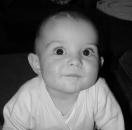
\includegraphics[width=0.5\textwidth]{baby_0}
                \caption{Das vorverarbeitete, ursprüngliche Bild.}
                \label{fig:imageseg-kkmpp-k-3-a}
        \end{subfigure}%
        \begin{subfigure}[b]{0.5\textwidth}
        		\centering
                
\includegraphics[width=0.5\textwidth]{baby_1}
                \caption{Das erste Cluster (das Gesicht).}
                \label{fig:imageseg-kkmpp-k-3-b}
        \end{subfigure}
        \begin{subfigure}[b]{0.5\textwidth}
        		\centering
                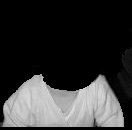
\includegraphics[width=0.5\textwidth]{baby_2}
                \caption{Das zweite Cluster (der Torso).}
                \label{fig:imageseg-kkmpp-k-3-c}
        \end{subfigure}%
        \begin{subfigure}[b]{0.5\textwidth}
        		\centering
                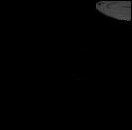
\includegraphics[width=0.5\textwidth]{baby_3}
                \caption{Das dritte Cluster (Fehler/Umgebung).}
                \label{fig:imageseg-kkmpp-k-3-d}
        \end{subfigure}
\caption{Mit \kkmpp{} segmentiertes Bild.}
\label{fig:imageseg-kkmpp}
\end{figure}
Abbildung~\ref{fig:imageseg-kkmpp} zeigt den graphischen Plot des berechneten Normalized Cut Clusterings von
Algorithmus \kkmpp. Auf den drei Clustern ist gut zu erkennen, dass unsere Clusteraufteilung hier gut funktioniert hat. Es
handelt sich um eine Beispielgrafik von der
Graclus-Webseite\footnote{\url{http://www.cs.utexas.edu/users/dml/Software/graclus.html} (Stand: 29.01.2015)}.
\absatz
Die Segmentierung einer einzelnen Grafik erfolgte nahezu unmittelbar. Um eine Vorstellung über die Leistungsfähigkeit des
Algorithmus in der Bildsegmentierung zu ermöglichen, haben wir ihn auf die
Extended Yale Face Database B (B+)\footnote{\url{http://vision.ucsd.edu/content/extended-yale-face-database-b-b}\\
(Stand: 29.01.2015)}~\cite{GeorghiadesBK01} angewandt. Dabei handelt es sich um eine Sammlung von 16128 Portrait-Fotos von
28 Menschen in 9 unterschiedlichen Positionen und 64 verschiedenen Belichtungsszenarien. Der gesamte Datensatz ist etwa
2 GB groß. Der Datensatz konnte mit \kkmpp{} in rund 50 Minuten verarbeitet werden. Unter Einsatz von METIS und mit
der spektralen Initialisierung dauerte die gesamte Verarbeitung rund 2 Stunden und 10 Minuten, also mehr als doppelt so lange.
Die "`Korrektheit"' der Gesichtserkennung konnte wegen der Anzahl der Bilder nicht vollständig ermittelt werden, da diese nur
durch menschlichen Augenschein verifiziert werden kann. Es ist nötig, bei einer Segmentierung zu prüfen, ob ein Cluster
dem Gesicht auf dem Foto entspricht.
In einer Stichprobe von 160 Bildern wurden 153 Bilder korrekt segmentiert, das entspricht einem Anteil von 96\%.
Bei der spektralen Methode wurden 157 Bilder korrekt segmentiert, was einem Anteil von 98\% entspricht.

\subsection{Kernmengenkonstruktion}
\label{subsection:experiment-coreset}

Unsere Variante der Kernmengenkonstruktion nennen wir in diesem Abschnitt verkürzt \CsTwo. Die empirische Evaluation
der "`Güte"' einer~(starken)~Kernmenge im Sinne ihrer Definition~\ref{def:strong-coreset}
beziehungsweise~\ref{def:coreset-with-offset} ist im Allgemeinen schwierig, da sich schlecht für alle möglichen Zentrenmengen
die jeweiligen Kosten vergleichen lassen. Neben der Messung der Laufzeiten geht man bezüglich der Qualitätsanalyse von Kernmengen
wie beispielsweise in~\cite{AckermannMRSLS12,FichtenbergerGSSS13} vor. Man berechnet einerseits die Kernmenge $S$ für die
Eingabepunktmenge $P$, wendet auf $S$ einen $k$-means-Algorithmus an und erhält eine Menge von $k$ Zentren
$C^1 = \{c_1^1, \dots, c_k^1\}$, für die sich $k$-means-Kosten $c^1$ in Bezug auf die Eingabepunktmenge $P$ ergeben.
Andererseits wendet man denselben $k$-means-Algorithmus direkt auf ganz $P$ an und erhält ebenfalls eine Zentrenmenge
$C^2 = \{c_1^2, \dots, c_k^2\}$, für die sich $k$-means-Kosten $c^2$ für $P$ ergeben. Die Kosten $c^1$ und $c^2$ lassen sich
vergleichen. Auf diese Weise wollen wir in diesem Abschnitt vorgehen. Dazu haben wir auf die Ausgaben der Kernmengen-Algorithmen,
die wir jeweils zehnmal ausgeführt haben,
den \kmpp-Algorithmus je zehnmal angewandt und die durchschnittlichen Kosten für den Vergleich
genommen. Insgesamt wurden also 100 Ausführungen gemessen.
Diese Methode der Evaluation ist zwar nicht allumfassend,
wir können jedoch den gesamten Algorithmus evaluieren und insbesondere die Leistungsfähigkeit der Kernmengenkonstruktion zur
Lösung des $k$-means-Problems bewerten.
\paragraph{Algorithmen.} Für einen Vergleich ziehen wir zunächst die Kernmengenkonstruktionen BICO~\cite{FichtenbergerGSSS13}
und \Skmpp~\cite{AckermannMRSLS12} heran. Beide Algorithmen sind state-of-the-art Datenstromalgorithmen zur Berechnung von
Kernmengen. Außerdem wollen wir auch hier wieder die Dlib-Implementierung von \kmpp{} zum Vergleich einsetzen, da wir in
unserer Konstruktion intensiven Gebrauch von der $D^2$-Gewichtung machen.
\paragraph{Datensätze.} Sowohl \kmpp{} als auch \CsTwo{} benötigen im Vergleich zu den Datenstromalgorithmen bereits auf Instanzen
mit mehreren hunderttausend Punkten vergleichsweise lange Ausführungszeiten. Wir beschränken uns daher in diesem Teil der
Evaluation auf mittelgroße Instanzen mit weniger als $10^6$ Punkten und insbesondere überschaubarer Dimensionsanzahl (bis
ca. $50$ Dimensionen). Tabelle~\ref{tbl:experiment-coresets-datasets} zeigt die Eigenschaften der ausgewählten Datensätze aus dem
UCI Machine Learning Repository.
\paragraph{Kernmengen-Größe.}
Eine asymptotische Größe von $\mathcal{O}(k)$ ist eine natürliche untere Schranke für die Größe einer Kernmenge, die wir
erreichen wollen. Wir orientieren uns in unseren Experimenten an~\cite{AckermannMRSLS12,FichtenbergerGSSS13}. In beiden Papieren
wurden in der experimentellen Auswertungen Kernmengen der Größe $200k$ konstruiert. Für die beiden Datensätze Spambase und
NYSK würden die Kernmengen bei einer Größe von $200k$ mehr Punkte enthalten als die Ursprungsmenge. Bei diesen beiden Datensätzen
haben wir daher Kernmengen der Größe $20k$ berechnet, um mehr Testwerte für einen umfassenderen Vergleich zu generieren.
Für die Evaluation unserer Konstruktion
ergibt sich die Herausforderung, die diversen Parameter so zu wählen, dass die berechnete Kernmenge in etwa diese
Größe annimmt. Wir können dies auf mehreren Wegen erreichen. Es ist beispielsweise möglich, schon bei
der initialen Partitionierung ein großes $c$ zu wählen (im Extremfall sogar schon hier $c=200$) und durch die maximale Tiefe
oder den Kostenfaktor $f$ dafür zu sorgen, dass nur bis zu einer geringen Tiefe partitioniert wird (oder im Extremfall
gar nicht weiter partitioniert wird). Alternativ können wir entsprechend auch ein kleines $c$ wählen und dafür größere
Werte von $d$ wählen, sodass wir initial nur wenige Teilmengen haben und in der rekursiven Partitionierung eine größere
Anzahl von Teilmengen erzielen.

\begin{table}[t]
\centering
\begin{tabular}{@{}ccc@{}} \toprule
	\textbf{Datensatz} & \textbf{Anzahl Punkte} & \textbf{Dimension} $d$ \\ \midrule
	Spambase & 4601 & 57 \\
	NYSK & 10421  & 7 \\
	Intrusion / KDD Cup 1999~\cite{AckermannMRSLS12} & 311078 & 34 \\
	Covertype & 581012 & 54 \\ \bottomrule
\end{tabular}
\caption{Eigenschaften der Datensätze aus~\cite{Lichman13} für die Evaluation von~\CsTwo.}
\label{tbl:experiment-coresets-datasets}
\end{table}

\paragraph{Clusteranzahl.} Wir wollen auch hier mit verschiedenen Werten für die Clusteranzahl $k$ arbeiten.
Dabei orientieren wir uns an den Experimenten aus~\cite{AckermannMRSLS12,FichtenbergerGSSS13}. Wir führen die Algorithmen
jeweils mit $k \in \{ 10, 30, 50 \}$ aus.

Wir geben bei den Ergebnistabellen immer den durchschnittlichen Wert für Kosten und Laufzeit von zehn
Ausführungen des \kmpp-Algorithmus für je zehn Ausführungen der Kernmengen-Algorithmen an. Bei den Kernmengen-Algorithmen
beziehen sich diese Werte auf die Ausführung von \kmpp{} unter
Eingabe der Kernmenge und bei \kmpp{} selbst auf die 100 Ausführungen auf der gesamten Punktmenge $P$. Für \CsTwo{} geben wir die
jeweiligen Parameter im Namen des Algorithmus an. Beispielsweise schreiben wir für $c = 200$, $d=/$, $f=/$ und $T=1$:
\CsTwo-c-200-d-/-f-/-T-1. Die Wahl von $d$ und $f$ ist hier irrelevant, da wegen $T$ nur initial partitioniert wird.
Dies deuten wir mit der Notation "`/"' an.
%\newpage
\begin{table}[h]
\centering
\begin{tabular}{@{}cccccc@{}} \toprule
	\textbf{Algorithmus} & $k$ & \multicolumn{4}{c}{\textbf{Datensatz}} \\
	\cmidrule(r){3-6} & 		& Spambase 				& NYSK 				& Intrusion 			& Covertype \\ \toprule
	\Skmpp 						& 10 & $7.85 \cdot 10^7$ & $5.67 \cdot 10^8$ & $1.27 \cdot 10^{13}$ & $3.43 \cdot 10^{11}$ \\
		 						& 30 & $1.24 \cdot 10^7$ & $4.22 \cdot 10^8$ & $4.29 \cdot 10^{11}$ & $1.57 \cdot 10^{11}$ \\
		 						& 50 & $6.29 \cdot 10^6$ & $6.12 \cdot 10^8$ & $1.11 \cdot 10^{11}$ & $1.15 \cdot 10^{11}$ \\
	\midrule
	BICO 						& 10 & $7.81 \cdot 10^7$ & $5.52 \cdot 10^8$ & $1.19 \cdot 10^{13}$ & $3.22 \cdot 10^{11}$ \\
			 					& 30 & $1.22 \cdot 10^7$ & $4.13 \cdot 10^8$ & $4.25 \cdot 10^{11}$ & $1.48 \cdot 10^{11}$ \\
		 						& 50 & $6.15 \cdot 10^6$ & $5.98 \cdot 10^8$ & $1.03 \cdot 10^{11}$ & $1.02 \cdot 10^{11}$ \\
	\midrule
	\kmpp 						& 10 & $8.71 \cdot 10^7$ & $6.09 \cdot 10^8$ & $1.75 \cdot 10^{13}$ & $3.42 \cdot 10^{11}$ \\
			 					& 30 & $1.34 \cdot 10^7$ & $4.98 \cdot 10^8$ & $4.96 \cdot 10^{11}$ & $1.54 \cdot 10^{11}$ \\
		 						& 50 & $6.68 \cdot 10^6$ & $7.01 \cdot 10^8$ & $1.29 \cdot 10^{11}$ & $1.13 \cdot 10^{11}$ \\
	\midrule
	\CsTwo-c-200-d-/-f-/-T-1	& 10 & $8.71 \cdot 10^7$ & $6.07 \cdot 10^8$ & $1.63 \cdot 10^{13}$ & $3.35 \cdot 10^{11}$ \\
			 					& 30 & - 				& $4.96 \cdot 10^8$ & $4.82 \cdot 10^{11}$ & $1.51 \cdot 10^{11}$ \\
		 						& 50 & - 				& $7.00 \cdot 10^8$	& $1.23 \cdot 10^{11}$ & $1.09 \cdot 10^{11}$ \\
	\midrule
	\CsTwo-c-1-d-50-f-1.3-T-3	& 10 & $8.33 \cdot 10^7$ & $5.92 \cdot 10^8$ & $1.59 \cdot 10^{13}$ & $3.31 \cdot 10^{11}$ \\
			 					& 30 & $1.30 \cdot 10^7$ & $4.88 \cdot 10^8$ & $4.75 \cdot 10^{11}$ & $1.48 \cdot 10^{11}$ \\
		 						& 50 & $6.59 \cdot 10^6$ & $6.89 \cdot 10^8$ & $1.19 \cdot 10^{11}$ & $1.06 \cdot 10^{11}$ \\
	\midrule
	\CsTwo-c-5-d-25-f-1.2-T-15	& 10 & $8.63 \cdot 10^7$ & $6.00 \cdot 10^8$ & $1.71 \cdot 10^{13}$ & $3.40 \cdot 10^{11}$ \\
			 					& 30 & $1.33 \cdot 10^7$ & $4.94 \cdot 10^8$ & $4.89 \cdot 10^{11}$ & $1.51 \cdot 10^{11}$ \\
		 						& 50 & $6.65 \cdot 10^6$ & $6.97 \cdot 10^8$ & $1.25 \cdot 10^{11}$ & $1.10 \cdot 10^{11}$ \\
	\midrule
	\CsTwo-c-50-d-10-f-1.4-T-10	& 10 & $8.22 \cdot 10^7$ & $5.85 \cdot 10^8$ & $1.52 \cdot 10^{13}$ & $3.30 \cdot 10^{11}$ \\
			 					& 30 & $1.28 \cdot 10^7$ & $4.80 \cdot 10^8$ & $4.70 \cdot 10^{11}$ & $1.47 \cdot 10^{11}$ \\
		 						& 50 & $6.49 \cdot 10^6$ & $6.81 \cdot 10^8$ & $1.17 \cdot 10^{11}$ & $1.09 \cdot 10^{11}$ \\
	\midrule
	\CsTwo-c-100-d-5-f-1.1-T-4	& 10 & $8.70 \cdot 10^7$ & $6.04 \cdot 10^8$ & $1.73 \cdot 10^{13}$ & $3.42 \cdot 10^{11}$ \\
			 					& 30 & $1.32 \cdot 10^7$ & $4.95 \cdot 10^8$ & $4.92 \cdot 10^{11}$ & $1.54 \cdot 10^{11}$ \\
		 						& 50 & - 				& $6.97 \cdot 10^8$ & $1.28 \cdot 10^{11}$ & $1.12 \cdot 10^{11}$ \\
	\bottomrule
\end{tabular}
\caption{Durchschnittliche Kosten der Algorithmen für $k \in \{ 10, 30, 50 \}$ (je kleiner, desto besser).}
\label{tbl:experiment-coresets-costs}
\end{table}
\newpage
\begin{table}[h]
\centering
\begin{tabular}{@{}cccccc@{}} \toprule
	\textbf{Algorithmus} & $k$ & \multicolumn{4}{c}{\textbf{Datensatz}} \\
	\cmidrule(r){3-6} & 		& Spambase 				& NYSK 				& Intrusion 			& Covertype \\ \toprule
	\Skmpp 						& 10 & $1.4$ 			& $2.7$ 			& $28.7$ 				& $115.2$ \\
		 						& 30 & $6.3$ 			& $9.3$ 			& $45.3$ 				& $170.5$ \\
		 						& 50 & $18.2$ 			& $25.2$ 			& $100.1$ 				& $290.2$ \\
	\midrule
	BICO 						& 10 & $0.1$ 			& $0.8$ 			& $7.6$ 				& $13.7$ \\
			 					& 30 & $0.1$ 			& $0.9$ 			& $9.8$ 				& $16.3$ \\
		 						& 50 & $0.1$ 			& $1.0$ 			& $12.1$ 				& $19.2$ \\
	\midrule
	\kmpp 						& 10 & $1.2$ 			& $2.9$ 			& $23.8$ 				& $181.2$ \\
			 					& 30 & $5.7$ 			& $10.2$ 			& $897.3$ 				& $2024.7$ \\
		 						& 50 & $13.3$ 			& $28.3$ 			& $644.0$ 				& $6922.9$ \\
	\midrule
	\CsTwo-c-200-d-/-f-/-T-1	& 10 & $1.2$			& $2.9$				& $22.6$ 				& $175.3$ \\
			 					& 30 & - 				& $10.0$			& $854.2$ 				& $1889.1$ \\
		 						& 50 & - 				& $27.8$			& $608.1$ 				& $6122.3$ \\
	\midrule
	\CsTwo-c-1-d-50-f-1.3-T-3	& 10 & $1.1$ 			& $2.5$ 			& $21.1$ 				& $155.3$ \\
			 					& 30 & $5.5$ 			& $9.1$ 			& $802.3$ 				& $1772.4$ \\
		 						& 50 & $12.9$ 			& $26.5$ 			& $577.2$ 				& $5532.1$ \\
	\midrule
	\CsTwo-c-5-d-25-f-1.2-T-15	& 10 & $1.0$ 			& $2.3$ 			& $19.9$ 				& $149.2$ \\
			 					& 30 & $5.2$ 			& $8.3$ 			& $763.7$ 				& $1566.3$ \\
		 						& 50 & $11.8$ 			& $23.2$ 			& $522.3$ 				& $5138.4$ \\
	\midrule
	\CsTwo-c-50-d-10-f-1.4-T-10	& 10 & $0.9$ 			& $1.8$ 			& $18.1$ 				& $121.3$ \\
			 					& 30 & $4.3$ 			& $7.6$ 			& $653.2$ 				& $1132.5$ \\
		 						& 50 & $9.9$ 			& $20.4$ 			& $434.1$ 				& $4237.2$ \\
	\midrule
	\CsTwo-c-100-d-5-f-1.1-T-4	& 10 & $1.0$ 			& $8.5$ 			& $20.6$ 				& $162.4$ \\
			 					& 30 & $5.1$ 			& $8.0$				& $788.1$ 				& $1802.4$ \\
		 						& 50 & - 				& $24.7$ 			& $554.3$ 				& $5322.1$ \\
	\bottomrule
\end{tabular}
\caption{Durchschnittliche Laufzeiten der Algorithmen für $k \in \{ 10, 30, 50 \}$ in Sekunden.}
\label{tbl:experiment-coresets-runtime}
\end{table}
Tabelle~\ref{tbl:experiment-coresets-costs} ist zu entnehmen, dass unsere Konstruktion mit allen Parametrisierungen bessere
$k$-means-Kosten erzielt als \kmpp. In der Spitze sind Verbesserungen von bis zu 10\% zu verzeichnen. Andererseits erzielen
die Datenstromalgorithmen \Skmpp und BICO durchweg noch geringere Kosten (in der Spitze bis rund 20\% weniger im Vergleich
zu \kmpp). Bei den Laufzeiten in Tabelle~\ref{tbl:experiment-coresets-runtime} ist deutlich zu erkennen, dass unsere
Kernmengenkonstruktion, die intensiven Gebrauch der $D^2$-Gewichtung macht, um einige Größenordnungen langsamer ist als die
state-of-the-art Datenstromalgorithmen. Die Läufe mit den geringsten Kosten und Laufzeiten sind jeweils bei $c = 50$ und
$d = 10$ und verbessern die Laufzeit von \kmpp{} um bis zu 40\%. Dies ist eine beachtliche Verbesserung.
Die dementsprechende Wahl der Parameter scheint empirisch sowohl für die Kosten als auch für die Laufzeit am besten geeignet
zu sein. 
\absatz
Es ist abzusehen, dass wir mit unserer Konstruktion keine
Laufzeiten in der Größenordnung der Datenstromalgorithmen erzielen können. Wir wollen stattdessen versuchen,
auch für die Kernmengenkonstruktion die Kernel Methode für alle Distanzberechnungen anzuwenden, um die erzielten Kosten zu
optimieren. Dazu setzen wir wieder einen Gauss-/RBF-Kernel mit $\sigma = 0.1$ ein. Für die Kernelvariante von \CsTwo{} schreiben
wir \KCsTwo.

\begin{table}[h]
\centering
\begin{tabular}{@{}cccccc@{}} \toprule
	\textbf{Algorithmus} & $k$ & \multicolumn{4}{c}{\textbf{Datensatz}} \\
	\cmidrule(r){3-6} & 		& Spambase 				& NYSK 				& Intrusion 			& Covertype \\ \toprule
	\Skmpp 						& 10 & $7.85 \cdot 10^7$ & $5.67 \cdot 10^8$ & $1.27 \cdot 10^{13}$ & $3.43 \cdot 10^{11}$ \\
		 						& 30 & $1.24 \cdot 10^7$ & $4.22 \cdot 10^8$ & $4.29 \cdot 10^{11}$ & $1.57 \cdot 10^{11}$ \\
		 						& 50 & $6.29 \cdot 10^6$ & $6.12 \cdot 10^8$ & $1.11 \cdot 10^{11}$ & $1.15 \cdot 10^{11}$ \\
	\midrule
	BICO 						& 10 & $7.81 \cdot 10^7$ & $5.52 \cdot 10^8$ & $1.19 \cdot 10^{13}$ & $3.22 \cdot 10^{11}$ \\
			 					& 30 & $1.22 \cdot 10^7$ & $4.13 \cdot 10^8$ & $4.25 \cdot 10^{11}$ & $1.48 \cdot 10^{11}$ \\
		 						& 50 & $6.15 \cdot 10^6$ & $5.98 \cdot 10^8$ & $1.03 \cdot 10^{11}$ & $1.02 \cdot 10^{11}$ \\
	\midrule
	\kmpp 						& 10 & $8.71 \cdot 10^7$ & $6.09 \cdot 10^8$ & $1.75 \cdot 10^{13}$ & $3.42 \cdot 10^{11}$ \\
			 					& 30 & $1.34 \cdot 10^7$ & $4.98 \cdot 10^8$ & $4.96 \cdot 10^{11}$ & $1.54 \cdot 10^{11}$ \\
		 						& 50 & $6.68 \cdot 10^6$ & $7.01 \cdot 10^8$ & $1.29 \cdot 10^{11}$ & $1.13 \cdot 10^{11}$ \\
	\midrule
	\KCsTwo-c-200-d-/-f-/-T-1	& 10 & $8.63 \cdot 10^7$ & $5.94 \cdot 10^8$ & $1.58 \cdot 10^{13}$ & $3.29 \cdot 10^{11}$ \\
			 					& 30 & - 				& $4.82 \cdot 10^8$ & $4.77 \cdot 10^{11}$ & $1.48 \cdot 10^{11}$ \\
		 						& 50 & - 				& $6.85 \cdot 10^8$	& $1.20 \cdot 10^{11}$ & $1.07 \cdot 10^{11}$ \\
	\midrule
	\KCsTwo-c-1-d-50-f-1.3-T-3	& 10 & $8.21 \cdot 10^7$ & $5.83 \cdot 10^8$ & $1.50 \cdot 10^{13}$ & $3.25 \cdot 10^{11}$ \\
			 					& 30 & $1.28 \cdot 10^7$ & $4.76 \cdot 10^8$ & $4.66 \cdot 10^{11}$ & $1.42 \cdot 10^{11}$ \\
		 						& 50 & $6.51 \cdot 10^6$ & $6.72 \cdot 10^8$ & $1.17 \cdot 10^{11}$ & $1.03 \cdot 10^{11}$ \\
	\midrule
	\KCsTwo-c-5-d-25-f-1.2-T-15	& 10 & $8.14 \cdot 10^7$ & $5.71 \cdot 10^8$ & $1.35 \cdot 10^{13}$ & $3.33 \cdot 10^{11}$ \\
			 					& 30 & $1.29 \cdot 10^7$ & $4.32 \cdot 10^8$ & $4.42 \cdot 10^{11}$ & $1.49 \cdot 10^{11}$ \\
		 						& 50 & $6.44 \cdot 10^6$ & $6.25 \cdot 10^8$ & $1.19 \cdot 10^{11}$ & $1.07 \cdot 10^{11}$ \\
	\midrule
	\KCsTwo-c-50-d-10-f-1.4-T-10& 10 & $7.83 \cdot 10^7$ & $5.58 \cdot 10^8$ & $1.22 \cdot 10^{13}$ & $3.25 \cdot 10^{11}$ \\
			 					& 30 & $1.23 \cdot 10^7$ & $4.19 \cdot 10^8$ & $4.27 \cdot 10^{11}$ & $1.44 \cdot 10^{11}$ \\
		 						& 50 & $6.27 \cdot 10^6$ & $5.99 \cdot 10^8$ & $1.07 \cdot 10^{11}$ & $1.03 \cdot 10^{11}$ \\
	\midrule
	\KCsTwo-c-100-d-5-f-1.1-T-4	& 10 & $8.52 \cdot 10^7$ & $5.97 \cdot 10^8$ & $1.68 \cdot 10^{13}$ & $3.36 \cdot 10^{11}$ \\
			 					& 30 & $1.30 \cdot 10^7$ & $4.91 \cdot 10^8$ & $4.88 \cdot 10^{11}$ & $1.51 \cdot 10^{11}$ \\
		 						& 50 & - 				& $6.90 \cdot 10^8$ & $1.24 \cdot 10^{11}$ & $1.10 \cdot 10^{11}$ \\
	\bottomrule
\end{tabular}
\caption{Durchschnittliche Kosten der Algorithmen für $k \in \{ 10, 30, 50 \}$ (je kleiner, desto besser).}
\label{tbl:experiment-coresets-kernelk-costs}
\end{table}
\newpage
\begin{table}[h]
\centering
\begin{tabular}{@{}cccccc@{}} \toprule
	\textbf{Algorithmus} & $k$ & \multicolumn{4}{c}{\textbf{Datensatz}} \\
	\cmidrule(r){3-6} & 		& Spambase 				& NYSK 				& Intrusion 			& Covertype \\ \toprule
	\Skmpp 						& 10 & $1.4$ 			& $2.7$ 			& $28.7$ 				& $115.2$ \\
		 						& 30 & $6.3$ 			& $9.3$ 			& $45.3$ 				& $170.5$ \\
		 						& 50 & $18.2$ 			& $25.2$ 			& $100.1$ 				& $290.2$ \\
	\midrule
	BICO 						& 10 & $0.1$ 			& $0.8$ 			& $7.6$ 				& $13.7$ \\
			 					& 30 & $0.1$ 			& $0.9$ 			& $9.8$ 				& $16.3$ \\
		 						& 50 & $0.1$ 			& $1.0$ 			& $12.1$ 				& $19.2$ \\
	\midrule
	\kmpp 						& 10 & $1.2$ 			& $2.9$ 			& $23.8$ 				& $181.2$ \\
			 					& 30 & $5.7$ 			& $10.2$ 			& $897.3$ 				& $2024.7$ \\
		 						& 50 & $13.3$ 			& $28.3$ 			& $644.0$ 				& $6922.9$ \\
	\midrule
	\KCsTwo-c-200-d-/-f-/-T-1	& 10 & $1.4$			& $3.3$				& $24.7$ 				& $217.5$ \\
			 					& 30 & - 				& $11.1$			& $922.1$ 				& $2007.0$ \\
		 						& 50 & - 				& $29.6$			& $673.3$ 				& $6536.7$ \\
	\midrule
	\KCsTwo-c-1-d-50-f-1.3-T-3	& 10 & $1.3$ 			& $2.8$ 			& $23.0$ 				& $171.1$ \\
			 					& 30 & $6.1$ 			& $9.9$ 			& $880.8$ 				& $1911.4$ \\
		 						& 50 & $13.8$ 			& $28.1$ 			& $607.9$ 				& $6072.1$ \\
	\midrule
	\KCsTwo-c-5-d-25-f-1.2-T-15	& 10 & $1.1$ 			& $2.6$ 			& $21.7$ 				& $164.3$ \\
			 					& 30 & $5.8$ 			& $8.9$ 			& $816.9$ 				& $1721.7$ \\
		 						& 50 & $12.9$ 			& $25.0$ 			& $578.2$ 				& $5649.1$ \\
	\midrule
	\KCsTwo-c-50-d-10-f-1.4-T-10& 10 & $1.0$ 			& $2.0$ 			& $19.9$ 				& $135.8$ \\
			 					& 30 & $4.6$ 			& $8.2$ 			& $702.1$ 				& $1281.9$ \\
		 						& 50 & $10.7$ 			& $22.2$ 			& $478.5$ 				& $4649.2$ \\
	\midrule
	\KCsTwo-c-100-d-5-f-1.1-T-4	& 10 & $1.1$ 			& $9.2$ 			& $22.9$ 				& $180.1$ \\
			 					& 30 & $5.5$ 			& $8.9$				& $872.2$ 				& $1993.5$ \\
		 						& 50 & - 				& $26.9$ 			& $612.1$ 				& $5911.8$ \\
	\bottomrule
\end{tabular}
\caption{Durchschnittliche Laufzeiten der Algorithmen für $k \in \{ 10, 30, 50 \}$ in Sekunden.}
\label{tbl:experiment-coresets-kernel-runtime}
\end{table}

\KCsTwo{} erzielt mit $c=50$ und $d=10$ durchweg Ergebnisse, die um einige Prozentpunkte besser sind als die für \kmpp{}
gemessenen Werte. Es ist naheliegend, dass wir somit unter Einsatz von \KCsTwo{} noch einmal eine Leistungssteigerung
in der Graphpartitionierung erreichen können.
Dies lässt sich in den folgenden beiden Tabellen~\ref{tbl:experiment-coreset-ncut-128}
und~\ref{tbl:experiment-coreset-ncut-runtime-128} für den Normalized Cut erkennen.
Die durchschnittliche Verbesserung beträgt hier in etwa 5-10\%.
\newpage
\begin{table}[h]
\centering
\begin{tabular}{@{}cccccc@{}} \toprule
	\textbf{Datensatz} & \textbf{Zufall} & \textbf{METIS} & \textbf{Spektral} & \textbf{\kkmpp{}} & \textbf{\KCsTwo{}} \\ \midrule
	BCSSTK31 	& 29.2 & 21.5 & 19.8 & 22 & 20.7  \\
	T60K 		& 6.9 & 5.4 & 4.8 & 5.8 & 5.0 \\
	598A 		& 16.1 & 14.3 & 12.4 & 13.5 & 12.4  \\
	144 		& 15.3 & 12.9 & 10.3 & 12.7 & 11.9  \\
	M14B 		& 24.2 & 21 & 18.7 & 21.7 & 20.2  \\
	AUTO 		& 12.1 & 9.9 & 8.2 & 9.5 & 8.8  \\
	\bottomrule
\end{tabular}
\caption{Durchschnittliche Normalized Cut Werte der Algorithmen für $k = 128$ (je kleiner, desto besser).}
\label{tbl:experiment-coreset-ncut-128}
\end{table}

\begin{table}[h]
\centering
\begin{tabular}{@{}cccccc@{}} \toprule
	\textbf{Datensatz} & \textbf{Zufall} & \textbf{METIS} & \textbf{Spektral} & \textbf{\kkmpp{}} &  \textbf{\KCsTwo{}} \\ \midrule
	BCSSTK31 	& 0.1 & 0.33 & 0.6 & 0.1 & 0.1 \\
	T60K 		& 0.1 & 0.18 & 0.3 & 0.1 & 0.1 \\
	598A 		& 0.4 & 0.97 & 1.5 & 0.5 & 0.5 \\
	144 		& 0.5 & 1.3 & 2.6 & 0.6 & 0.5 \\
	M14B 		& 0.8 & 2.0 & 3.8 & 1.1 & 1.0 \\
	AUTO 		& 1.9 & 4.2 & 7.3 & 2.9 & 2.7 \\
	\bottomrule
\end{tabular}
\caption{Durchschnittliche Laufzeiten der Algorithmen für Normalized Cut mit $k = 128$.}
\label{tbl:experiment-coreset-ncut-runtime-128}
\end{table}
\section{Zusammenfassung}
\label{section:conclusion}

Die Kernel Methode ist eine wirkungsvolle Technik in der Clusteranalyse. Ihr Einsatz erlaubt es, die Effektivität von Verfahren
signifikant zu steigern, die auf die lineare Separierung von Clustern beschränkt sind. Angewandt auf den $k$-means-Algorithmus
erhält man den Kernel-$k$-means-Algorithmus, mit dem sich beispielsweise das Graph\-partitionierungsproblem lösen lässt, wie wir
in Abschnitt~\ref{subsection:wkkm-graphcut-graphclustering} erläutert haben.
\absatz
Der \kmpp-Algorithmus sieht eine geschicktere Wahl der initialen Zentren für den $k$-means-Algorithmus vor.
Wir haben die Kernel Methode auf \kmpp{} angewandt und den resultierenden \kkmpp-Algorithmus vorgestellt.
Dabei konnten wir zeigen, dass die $\mathcal{O}(\log k)$-Approximationseigenschaft von \kmpp{} erhalten bleibt.
Bislang haben in der Graphpartitionierung spektrale Verfahren die qualitativ besten Ergebnisse geliefert.
Diese bringen jedoch wegen der nötigen Eigenvektorberechnungen hohe Laufzeiten mit sich.
Mit \kkmpp{} war es uns möglich, Graphpartitionierungen ohne spektrale Techniken zu berechnen, die qualitativ kompetitiv zu
den bisherigen Verfahren sind. Wir konnten jedoch gleichzeitig die Laufzeiten um einen Faktor zwei verbessern. Dies ist besonders
erfreulich, wenn man bedenkt, dass das modifizierte Framework Graclus die derzeit vielleicht schnellste quelloffene
Software im Bereich der Graphpartitionierung ist, die von einer Reihe von quelloffenen Bildverarbeitungsprogrammen eingesetzt wird.
\absatz
Wir haben zudem eine Variante der Kernmengenkonstruktion von Feldman, Schmidt und Sohler~\cite{FeldmanSS13} vorgestellt,
die in den Experimenten praktikable Qualität und Laufzeit aufweist. Insbesondere die Kernel-basierte Variante liefert bessere
Ergebnisse als der \kmpp-Algorithmus. Mit der Kernmengenkonstruktion war es uns möglich, den Kernel-$k$-means-basierten 
Algorithmus zur Graphpartitionierung noch einmal zu verbessern.
\absatz
Über diese Arbeit hinaus wäre es sicherlich interessant, zu untersuchen, ob die Kernel Methode auch auf andere $k$-means-Algorithmen
angewandt werden kann und ob dies zu Verbesserungen führt.

Für die Kernmengenkonstruktion haben wir in der Einleitung eine mögliche Anwendung in der verteilten Clusteranalyse erwähnt.
Es wäre daher sicherlich interessant, eine verteilte Variante der Konstruktion zu implementieren und diese dann auf verteilt
vorliegenden zu clusternden Daten zu untersuchen. Dabei sollte der Algorithmus nicht nur auf einigen wenigen Maschinen ausgeführt
werden sondern auf 16 oder mehr Knoten, um die Leistungsfähigkeit in verteilten System zu analysieren.

% Anhänge

% Literatur
\emptypagenumbered
\addcontentsline{toc}{section}{Literatur}
\bibliographystyle{alphadin}
\bibliography{bib}
\nocite{*}

% Erklärung
\iftoggle{erklaerung}{
	\emptypagenumbered
	%\emptypagenumbered
	%\markboth{}{ERKLÄRUNG}
	\addcontentsline{toc}{section}{Erklärung}
	%Hiermit versichere ich, dass ich die vorliegende Arbeit selbstständig verfasst habe und keine
anderen als die angegebenen Quellen und Hilfsmittel verwendet sowie Zitate kenntlich gemacht habe.\\\\
Dortmund, den \today \\\\\\\\
Lukas Pradel
	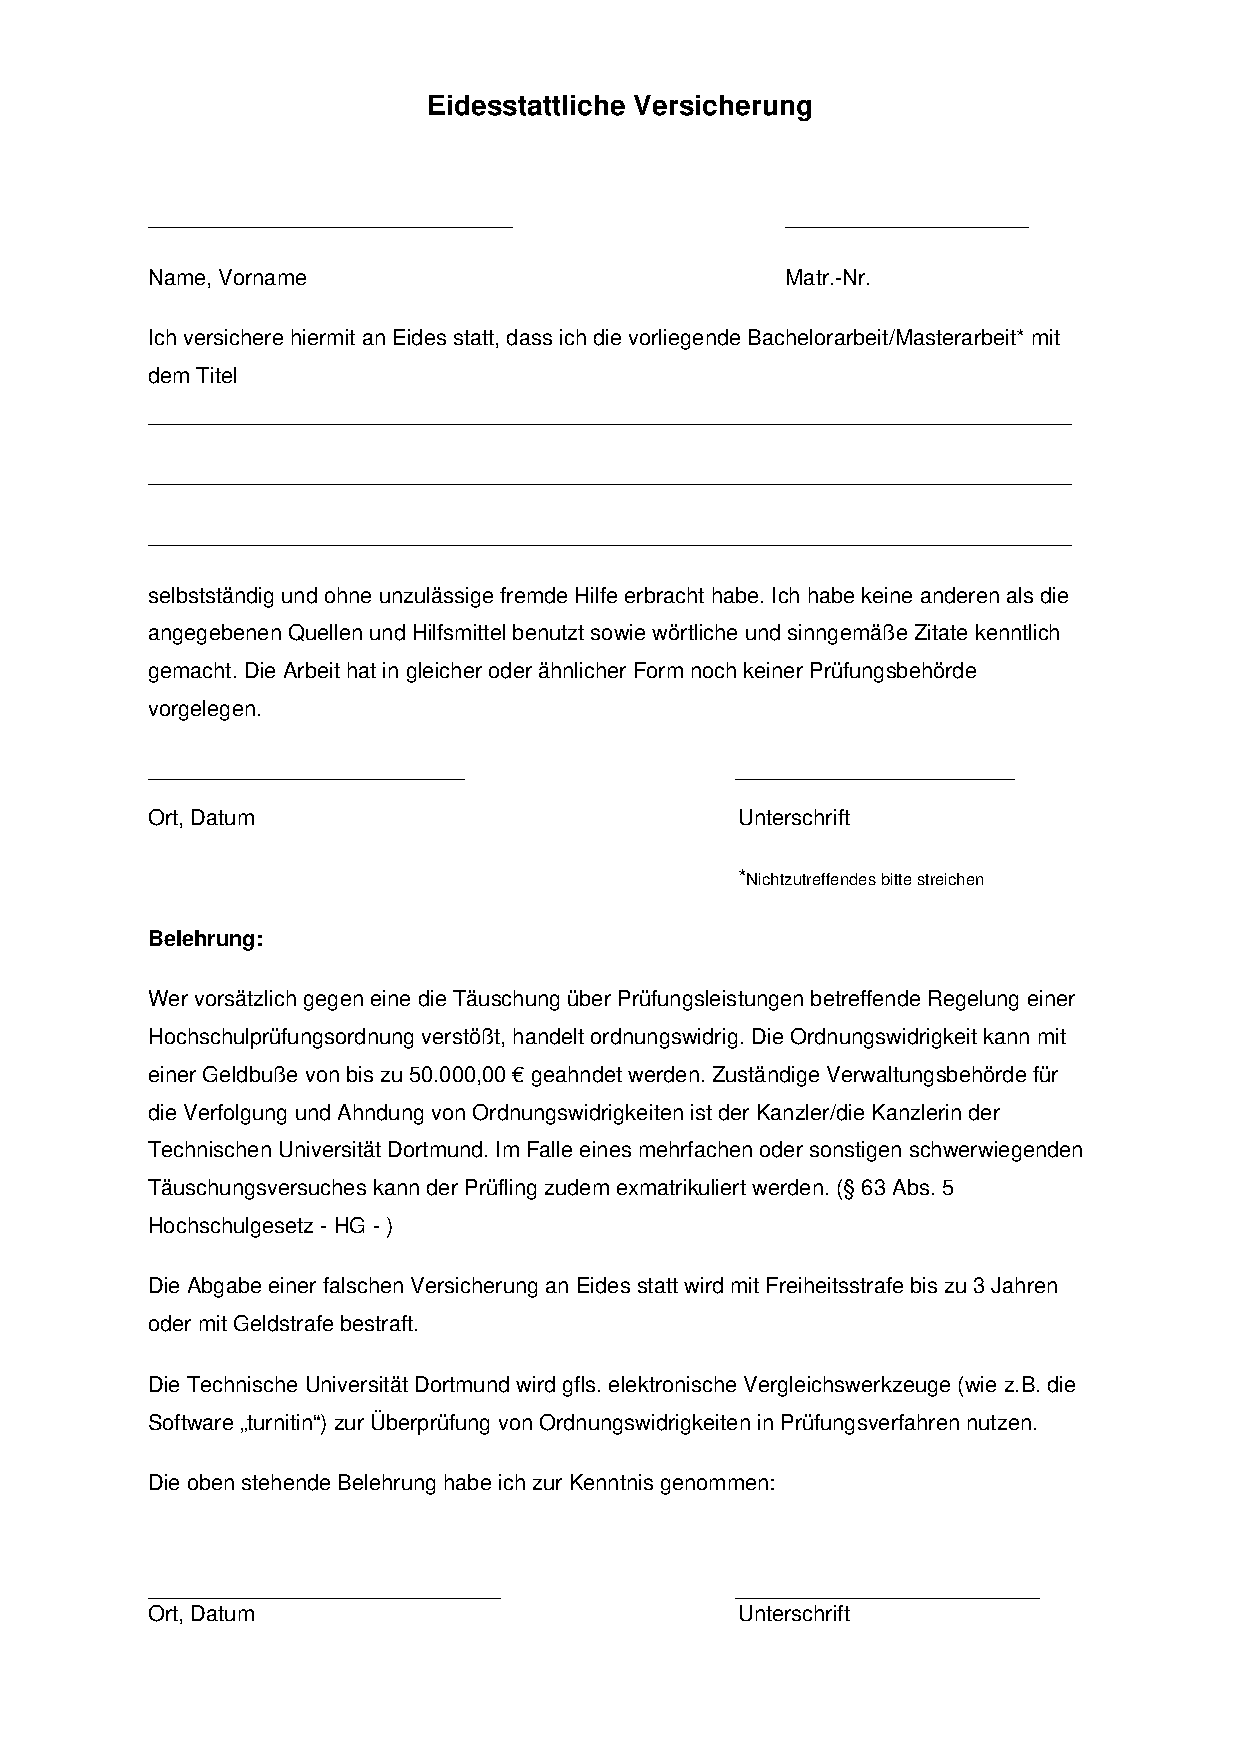
\includepdf[pages={1}]{appendices/erklaerung.pdf}
}

\emptypagenumbered

\end{document}